
\documentclass[conference]{IEEEtran}
\IEEEoverridecommandlockouts

\usepackage{cite}
\usepackage{amsmath,amssymb}
\usepackage{booktabs}
\usepackage{array}
\usepackage{tabularx}
\usepackage{multirow}
\usepackage{makecell}
\usepackage{enumitem}
\usepackage{url}
\usepackage[hidelinks]{hyperref}
\usepackage{listings}
\usepackage{xcolor}
\usepackage{tikz}
\usetikzlibrary{positioning,arrows.meta,shapes.geometric,fit,calc}

\newcolumntype{Y}{>{\raggedright\arraybackslash}X}
\newcolumntype{L}[1]{>{\raggedright\arraybackslash}p{#1}}
\renewcommand{\arraystretch}{1.16}
\lstdefinelanguage{PlantUML}{
  morekeywords={start,stop,if,then,else,endif,actor,participant,boundary,control,database,cloud,rectangle,package,title,skinparam,left,right,direction,autonumber,usecase,as},
  sensitive=false,
  morecomment=[l]{'},
  morestring=[b]",
}
\lstset{
  language=PlantUML,
  basicstyle=\scriptsize\ttfamily,
  breaklines=true,
  columns=fullflexible,
  frame=single,
  numbers=left,
  numberstyle=\tiny,
  captionpos=b,
  showstringspaces=false,
  tabsize=2
}

\title{Behavioral UML Documentation and Hyperledger Fabric Mapping of Procurement Business Processes for an E-Procurement Service}

\author{\IEEEauthorblockN{Harith Irfan}
\IEEEauthorblockA{Independent Research Draft\\
Email: asynashen@gmail.com}}

\begin{document}
\maketitle

\begin{abstract}
Procurement work is often executed through fragmented approvals, email-based quotations, manual purchase-order preparation, paper delivery confirmations, spreadsheet-based evaluations, and accounts-payable exception handling. These handoffs make it difficult for engineers to determine which process flows should be digitized, automated, or supported by tamper-evident records. This paper presents an IEEE-style behavioral modeling study of procurement business processes for an e-procurement service integrated with Hyperledger Fabric. The study identifies actors, terminology, process objectives, triggers, inputs, outputs, normal flows, alternative flows, exception flows, business rules, inefficiencies, and streamlining opportunities. It then maps each process to frontend interfaces, backend services, database entities, blockchain assets, Fabric chaincode functions, and ledger events. The paper provides a UML-oriented documentation package using use case, activity, sequence, state-machine, and component-level representations. The analysis argues that blockchain is not a universal replacement for procurement databases; rather, it is most defensible for multi-party trust, non-repudiation, traceability, and auditability of critical procurement milestones. Sensitive documents and detailed commercial data should remain off-chain, while ledger entries should store lifecycle states, hashes, identities, timestamps, and events.
\end{abstract}

\begin{IEEEkeywords}
e-procurement, business process analysis, UML, activity diagram, sequence diagram, Hyperledger Fabric, blockchain, chaincode, procurement audit, procure-to-pay, source-to-contract
\end{IEEEkeywords}

\section{Introduction}
Procurement is a cross-functional business capability that connects demand identification, supplier selection, ordering, receiving, invoicing, payment, compliance, and supplier performance management. In many organizations, the process is only partially digitized: requests are created in email, approvals occur through informal messages, quotation comparisons are performed in spreadsheets, purchase orders are rekeyed into finance systems, and invoice matching requires manual reconciliation. These practices increase cycle time, data inconsistency, maverick spending, contract leakage, invoice exceptions, and audit cost. Prior procurement research and benchmark evidence show that process redesign, automation, data quality, system compliance, and supplier adoption strongly influence e-procurement value \cite{croom2007,vaidya2006,brandon2011,apqc2019,worldbank2023}.

The research task addressed in this paper is: how can selected procurement business processes be documented, visualized, and analyzed using behavioral UML diagrams so that engineers can understand current process flow, identify inefficiencies, and map each process to a possible e-procurement service architecture supported by frontend interfaces, backend services, databases, and Hyperledger Fabric blockchain networks? The contribution is a structured process catalog, use case specification, UML diagram inventory, and architecture mapping that future software engineers can use as a requirements baseline.

This paper is not a full software implementation specification. It does not prescribe a specific ERP product, cloud vendor, programming language, database engine, or legal compliance regime. It models a generic medium-to-large buying organization. Organization-specific facts, thresholds, supplier categories, approval limits, tax rules, and payment regulations must be configured during implementation.

\section{Task Interpretation, Scope, and Assumptions}
The task is interpreted as a business-process and system-design study rather than a code build. The selected processes span source-to-contract (S2C), procure-to-pay (P2P), supplier management, accounts payable, compliance, and exception handling. The design objective is educational: business readers should understand process meaning and engineering readers should see how process events become system services, data records, and Fabric ledger events.

The assumed process scope includes the fourteen processes listed in the prompt and one additional process: supplier performance and contract closeout. It is included because procurement does not end at payment; engineers need feedback loops from delivery quality, disputes, invoice exceptions, and contract closeout to future supplier selection. The main assumptions are: (i) the buyer organization controls the e-procurement application; (ii) suppliers access the system through a portal; (iii) an operational database remains the source for mutable application data and large documents; (iv) Hyperledger Fabric stores asset lifecycle events, hashes, selected non-sensitive metadata, and audit states; and (v) private data collections may be used where subsets of organizations need restricted ledger-side data sharing.

\section{Background and Related Concepts}
\subsection{Procurement, S2C, and P2P}
Procurement is the organized acquisition of goods and services needed by an organization. In a systems context, S2C includes requirement definition, market analysis, RFQ or tendering, supplier evaluation, negotiation, award, and contract creation. P2P includes purchase requisition, approval, purchase order, goods or service receipt, invoice verification, and payment. A P2P definition normally treats requisition, sourcing or ordering, receiving, invoicing, and payment as one connected flow \cite{ibm_p2p,sap_p2p}.

\subsection{Behavioral UML for Process Understanding}
UML is a standard graphical language for visualizing and documenting software-intensive systems \cite{omg_uml}. This paper emphasizes behavioral diagrams because procurement is primarily a workflow problem: use case diagrams identify externally visible goals; activity diagrams show control flow and decisions; sequence diagrams show messages among actors and system components; and state-machine diagrams show lifecycle states of business assets such as VendorProfile, RFQ, PurchaseOrder, Invoice, and PaymentApproval.

\subsection{Hyperledger Fabric as Procurement Audit Infrastructure}
Hyperledger Fabric is an enterprise-oriented permissioned distributed ledger platform \cite{fabric_main}. Fabric peers host ledgers and chaincode, client applications submit transaction proposals, endorsement policies specify which organizations must endorse, and the ordering service orders transactions into blocks for peer validation and commit \cite{fabric_peers,fabric_ordering}. The Membership Service Provider (MSP) and certificate authorities establish trusted identities for organizations and users \cite{fabric_msp,fabric_security}. Fabric private data collections can keep sensitive data visible only to an authorized subset of organizations while still anchoring hashes on the channel ledger \cite{fabric_private}.

\begin{table*}[t]
\caption{Glossary of Business and Blockchain Terms}
\label{tab:glossary}
\scriptsize
\begin{tabularx}{\textwidth}{|L{3.0cm}|Y|}
\hline
\textbf{Term} & \textbf{Explanation for business and engineering audiences} \\ \hline
Procurement & The organizational process of obtaining goods and services needed to operate, including sourcing, ordering, receiving, invoicing, and supplier management. \\ \hline
Purchase requisition & An internal request to buy goods or services before a purchase order is issued; it captures need, quantity, budget, and justification. \\ \hline
Purchase order & A formal buyer document sent to a supplier specifying items, quantities, prices, delivery terms, and payment terms. \\ \hline
Request for quotation (RFQ) & A sourcing document asking suppliers to submit price and delivery offers for defined requirements. \\ \hline
Supplier onboarding & The process of collecting, verifying, and approving supplier identity, tax, bank, compliance, and risk data. \\ \hline
Approval workflow & A rule-based sequence of authorization tasks that ensures spending is approved by the correct roles and thresholds. \\ \hline
Three-way matching & The control that compares purchase order, goods receipt or service confirmation, and invoice before payment. \\ \hline
Invoice verification & The accounts-payable process of validating invoice data, tax details, supplier identity, duplicates, and matching results. \\ \hline
Audit trail & A chronological evidence record showing who performed each action, when, and with what data or decision. \\ \hline
Smart contract & Executable business logic on a blockchain. In Hyperledger Fabric, smart contracts are implemented as chaincode. \\ \hline
Chaincode & Fabric application code that validates transactions and reads or writes ledger state. \\ \hline
Ledger & The shared record of validated transactions and current asset state maintained by Fabric peers on a channel. \\ \hline
Endorsement policy & A Fabric rule defining which organizations or peers must endorse a transaction before it can be ordered and committed. \\ \hline
Ordering service & The Fabric service that orders endorsed transactions into blocks and distributes them to peers for validation and commit. \\ \hline
Peer node & A Fabric node that hosts ledgers and chaincode, endorses transaction proposals, and commits valid blocks. \\ \hline
Certificate Authority & The authority that issues cryptographic identities used by participants in the permissioned network. \\ \hline
Membership Service Provider (MSP) & The Fabric mechanism that defines trusted identities, roles, and organizations allowed to participate in channels and policies. \\ \hline
Immutability & The property that committed ledger entries are append-only and tamper-evident after validation. \\ \hline
Non-repudiation & A control objective where a participant cannot plausibly deny a signed action or submitted transaction. \\ \hline
Traceability & The ability to follow the lifecycle of procurement assets across requisition, RFQ, quotation, PO, delivery, invoice, payment, and audit. \\ \hline
\end{tabularx}
\end{table*}

\section{Methodology}
The method follows eight steps. First, procurement processes are identified from the domain scope and from common S2C/P2P practice. Second, actors and stakeholders are defined. Third, a business glossary normalizes terms so that analysts and engineers use the same vocabulary. Fourth, each process is decomposed into objective, trigger, actors, preconditions, inputs, outputs, normal flow, alternative flow, exception flow, rules, pain points, e-procurement opportunity, and blockchain opportunity. Fifth, process outputs are mapped to system components: frontend screens, backend services, database entities, Fabric transactions, chaincode functions, and ledger events. Sixth, UML behavioral representations are prepared as PlantUML source. Seventh, current manual or semi-manual processes are compared with a digitized process supported by workflow automation and ledger-backed audit. Finally, limitations and recommendations are derived.

\section{Overall Business Process Context}
\subsection{Actor and Stakeholder Analysis}
Table~\ref{tab:actors} lists the main actors. The architecture distinguishes human actors from system components. A supplier, for example, is a business actor, while the supplier portal is a frontend interface. Similarly, Hyperledger Fabric is not a human stakeholder but a network infrastructure that enforces identity-aware transaction validation and audit-state replication.

\begin{table*}[t]
\caption{Actors and Stakeholders}
\label{tab:actors}
\scriptsize
\begin{tabularx}{\textwidth}{|L{3.0cm}|Y|Y|Y|}
\hline
\textbf{Actor} & \textbf{Business role} & \textbf{System permissions} & \textbf{Typical data handled} \\ \hline
Requesting Department/User & Identifies the business need, creates requisitions, confirms services, and supplies specifications. & Create requisition; view status; provide clarifications; confirm service acceptance. & Need description, quantity, cost center, justification, service acceptance. \\ \hline
Approver/Manager & Authorizes spending and exceptions based on budget, authority, and policy. & Approve/reject/return requests; delegate authority; approve exceptions. & Approval decision, comments, timestamp, delegation evidence. \\ \hline
Procurement Officer & Runs sourcing, supplier selection, RFQ, PO, contract, and supplier performance activities. & Create RFQs, evaluate bids, issue POs, manage contracts and exceptions. & RFQ data, award recommendation, PO, contract terms, case decisions. \\ \hline
Vendor/Supplier & Registers profile, submits quotations, acknowledges POs, delivers goods/services, and submits invoices. & Self-service onboarding; bid submission; PO acknowledgement; invoice status. & Company data, quotation, delivery note, invoice, dispute evidence. \\ \hline
Finance/AP Officer & Verifies invoices, matches PO/receipt/invoice, approves payments, and maintains payment controls. & Invoice verification, payment approval, exception routing. & Invoice status, match result, payment approval, bank validation reference. \\ \hline
Receiving Officer/Service Owner & Confirms delivery quantity, quality, and service completion. & Record goods receipt; accept/reject delivery; upload evidence. & Goods receipt, inspection result, photos, service acceptance. \\ \hline
Auditor/Compliance Officer & Reviews policy compliance, risk, audit evidence, and remediation. & Read-only evidence packs; create findings; close remediation. & Audit findings, exception classification, control test evidence. \\ \hline
System Administrator & Manages roles, workflow rules, integration configuration, and access controls. & Maintain users/roles/rules; configure APIs and Fabric connection. & User-role mapping, approval matrix, channel policy configuration. \\ \hline
Hyperledger Fabric Network & Provides permissioned ledger, chaincode, endorsement, ordering, and immutable event history. & Endorse and commit transactions; emit events; enforce asset lifecycle rules. & Asset state, transaction log, event stream, private-data hash. \\ \hline
\end{tabularx}
\end{table*}

\subsection{Simplified Actor-System Interaction Model}
Fig.~\ref{fig:contexttikz} provides a simplified architecture view. It is intentionally high-level because the purpose is to make process responsibilities visible before implementation details are selected.

\begin{figure*}[t]
\centering
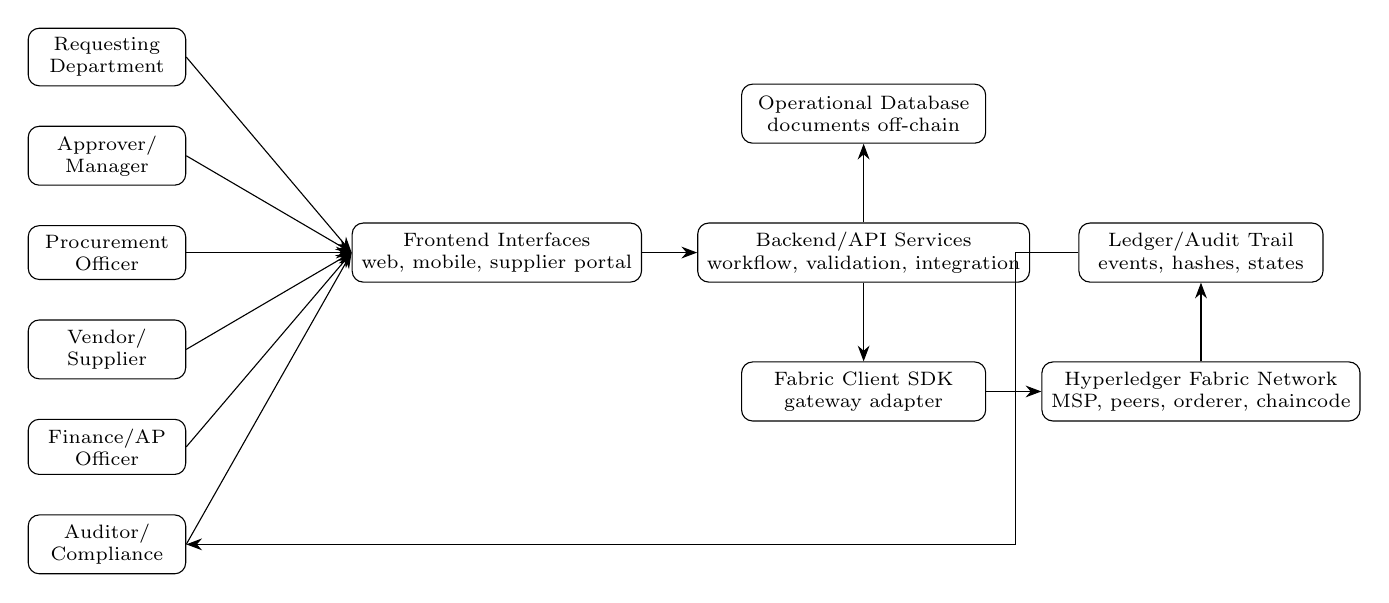
\begin{tikzpicture}[
  font=\scriptsize,
  actor/.style={draw, rounded corners, align=center, minimum width=2.0cm, minimum height=0.55cm},
  layer/.style={draw, rounded corners, align=center, minimum width=3.1cm, minimum height=0.75cm},
  arrow/.style={-{Stealth[length=2mm]}, line width=0.4pt},
  node distance=0.5cm and 0.7cm
]
\node[actor] (req) {Requesting\\Department};
\node[actor, below=of req] (app) {Approver/\\Manager};
\node[actor, below=of app] (proc) {Procurement\\Officer};
\node[actor, below=of proc] (sup) {Vendor/\\Supplier};
\node[actor, below=of sup] (fin) {Finance/AP\\Officer};
\node[actor, below=of fin] (aud) {Auditor/\\Compliance};

\node[layer, right=2.1cm of proc] (ui) {Frontend Interfaces\\web, mobile, supplier portal};
\node[layer, right=of ui] (api) {Backend/API Services\\workflow, validation, integration};
\node[layer, above=1.0cm of api] (db) {Operational Database\\documents off-chain};
\node[layer, below=1.0cm of api] (sdk) {Fabric Client SDK\\gateway adapter};
\node[layer, right=of sdk] (fab) {Hyperledger Fabric Network\\MSP, peers, orderer, chaincode};
\node[layer, above=1.0cm of fab] (ledger) {Ledger/Audit Trail\\events, hashes, states};

\foreach \x in {req,app,proc,sup,fin,aud} \draw[arrow] (\x.east) -- (ui.west);
\draw[arrow] (ui) -- (api);
\draw[arrow] (api) -- (db);
\draw[arrow] (api) -- (sdk);
\draw[arrow] (sdk) -- (fab);
\draw[arrow] (fab) -- (ledger);
\draw[arrow] (ledger.west) -- ++(-0.8,0) |- (aud.east);
\end{tikzpicture}
\caption{Simplified actor-system interaction model. Human actors use frontend interfaces; backend services validate workflow and persist operational records; Fabric records selected procurement states, hashes, and events for auditability.}
\label{fig:contexttikz}
\end{figure*}

\section{Business Process Catalog}
Table~\ref{tab:catalog} catalogs the processes in scope. Blockchain relevance is intentionally qualified. A high blockchain relevance does not mean all data should be on-chain; it means the process has valuable audit, non-repudiation, cross-party, or lifecycle-state evidence.

\begin{table*}[!t]
\caption{Business Process Catalog (Part 1 of 3)}
\label{tab:catalog}
\tiny
\begin{tabularx}{\textwidth}{|L{0.85cm}|L{2.3cm}|L{2.1cm}|L{2.6cm}|Y|L{2.0cm}|Y|Y|}
\hline
\textbf{Process ID} & \textbf{Business Process Name} & \textbf{Primary Actor} & \textbf{Supporting Actors} & \textbf{Trigger} & \textbf{Main Output} & \textbf{Blockchain Relevance} & \textbf{Streamlining Opportunity} \\ \hline
BP01 & Vendor Registration and Onboarding & Vendor/Supplier & Procurement Officer, Compliance Officer, System Administrator & New supplier wishes to transact or is invited by procurement & Approved VendorProfile or rejection notice & High: identity, compliance status, bank-data attestation hash, immutable onboarding history & Supplier self-service, automated validation, risk scoring, duplicate detection \\ \hline
BP02 & Purchase Requisition Creation & Requesting Department & Procurement Officer, Budget Owner & Business need for goods or services & Submitted PurchaseRequisition & Medium: hash of submitted requisition, requester identity, budget category, version history & Guided buying, catalog selection, budget validation, form standardization \\ \hline
BP03 & Purchase Request Approval & Approver/Manager & Requesting Department, Procurement Officer, Finance Officer & Submitted requisition requires approval & Approved or rejected requisition & High: approval decision, digital signature, authority level, timestamp & Rule-based routing, escalation, delegation, threshold controls \\ \hline
BP04 & Request for Quotation Preparation and Publication & Procurement Officer & Requesting Department, Supplier, Approver & Approved requisition requires competitive quotation or tendering & Published RFQ/RFP/Tender package & High: RFQ publication time, eligible suppliers, immutable terms hash & Template reuse, supplier invitation, electronic bid windows, evaluation rules \\ \hline
BP05 & Supplier Quotation Submission & Vendor/Supplier & Procurement Officer, System Administrator & Supplier receives RFQ invitation or public tender access & Submitted Quotation & High: bid timestamp, confidentiality hash, supplier identity, anti-tampering evidence & Electronic bid submission, deadline enforcement, sealed-bid controls \\ \hline
\end{tabularx}
\end{table*}

\begin{table*}[!t]
\caption{Business Process Catalog (Part 2 of 3)}
\label{tab:catalog-2}
\tiny
\begin{tabularx}{\textwidth}{|L{0.85cm}|L{2.3cm}|L{2.1cm}|L{2.6cm}|Y|L{2.0cm}|Y|Y|}
\hline
\textbf{Process ID} & \textbf{Business Process Name} & \textbf{Primary Actor} & \textbf{Supporting Actors} & \textbf{Trigger} & \textbf{Main Output} & \textbf{Blockchain Relevance} & \textbf{Streamlining Opportunity} \\ \hline
BP06 & Quotation Evaluation and Supplier Award & Procurement Officer & Evaluation Committee, Requesting Department, Approver, Auditor & RFQ closes and quotations are available for evaluation & Award recommendation and selected supplier & High: evaluation scoring hash, award decision, committee approvals, conflict-of-interest evidence & Evaluation templates, scoring matrix, comparative analytics, approval routing \\ \hline
BP07 & Purchase Order Generation and Supplier Acceptance & Procurement Officer & Supplier, Finance Officer, Requesting Department & Approved award, catalog requisition, or contract release & Issued and acknowledged PurchaseOrder & High: PO commitment, supplier acknowledgement, version history & Auto-generation from requisition/award, electronic dispatch, acknowledgement tracking \\ \hline
BP08 & Contract Creation and Approval & Procurement Officer & Legal Officer, Supplier, Approver, Compliance Officer & Award requires formal contract or framework agreement & Approved and active Contract & High: contract hash, approval signatures, version and amendment trail & Template clauses, approval workflow, obligation extraction, renewal alerts \\ \hline
BP09 & Goods or Service Delivery Confirmation & Receiving Officer & Supplier, Requesting Department, Procurement Officer & Supplier delivers goods or completes service milestone & GoodsReceipt or ServiceAcceptance record & High: delivery confirmation, acceptance/rejection, quantity and timestamp evidence & Mobile receiving, barcode/QR capture, automated PO matching \\ \hline
BP10 & Invoice Submission & Vendor/Supplier & Finance Officer, Procurement Officer & Supplier has delivered goods/services and seeks payment & Submitted Invoice & Medium-High: invoice hash, submission timestamp, supplier identity, duplicate prevention & E-invoicing, PO flip, mandatory validation, invoice status self-service \\ \hline
\end{tabularx}
\end{table*}

\begin{table*}[!t]
\caption{Business Process Catalog (Part 3 of 3)}
\label{tab:catalog-3}
\tiny
\begin{tabularx}{\textwidth}{|L{0.85cm}|L{2.3cm}|L{2.1cm}|L{2.6cm}|Y|L{2.0cm}|Y|Y|}
\hline
\textbf{Process ID} & \textbf{Business Process Name} & \textbf{Primary Actor} & \textbf{Supporting Actors} & \textbf{Trigger} & \textbf{Main Output} & \textbf{Blockchain Relevance} & \textbf{Streamlining Opportunity} \\ \hline
BP11 & Invoice Verification and Three-Way Matching & Finance Officer & Procurement Officer, Receiving Officer, Supplier & Invoice is submitted and ready for validation & Matched invoice, exception case, or rejection & High: match result, tolerance decision, exception resolution history & Automated two-way/three-way matching, tolerance rules, exception queues \\ \hline
BP12 & Payment Approval and Payment Instruction & Finance Officer & Approver/Manager, Supplier, Treasury/Bank Interface & Invoice is matched or exception approval is complete & Approved payment instruction and payment status & Medium-High: approval timestamp, payer identity, payment authorization hash & Payment approval queues, segregation checks, bank integration, supplier status visibility \\ \hline
BP13 & Procurement Audit and Compliance Review & Auditor/Compliance Officer & Procurement Officer, Finance Officer, System Administrator & Scheduled audit, risk alert, dispute, management review, or regulatory request & Audit findings, compliance status, remediation actions & Very high: immutable process chronology, evidence hashes, chain of custody & Digital audit trails, automated exception reports, evidence dashboards \\ \hline
BP14 & Dispute or Exception Handling & Procurement Officer & Supplier, Finance Officer, Receiving Officer, Auditor, Approver & Mismatch, rejected delivery, supplier protest, invoice exception, contract dispute, or policy violation & Resolved exception, corrective action, or escalated dispute & High: dispute timeline, evidence hashes, decisions, settlement record & Exception case management, SLA tracking, root-cause analytics \\ \hline
BP15 & Supplier Performance and Contract Closeout & Procurement Officer & Requesting Department, Supplier, Compliance Officer, Auditor & Delivery completion, contract milestone, periodic review, or contract expiry & Supplier scorecard, closeout record, renewal/termination decision & Medium-High: performance score hash, milestone completion, closeout evidence & Automated scorecards, KPI tracking, renewal alerts, performance feedback loops \\ \hline
\end{tabularx}
\end{table*}

\section{Use Case Specifications}
Table~\ref{tab:usecases} summarizes the use case specifications. The table is compressed for IEEE layout; the narrative subsections that follow provide detailed process interpretation.

\begin{table*}[!t]
\caption{Use Case Specification Summary (Part 1 of 5)}
\label{tab:usecases}
\tiny
\begin{tabularx}{\textwidth}{|L{0.75cm}|L{1.8cm}|L{1.6cm}|Y|Y|Y|Y|Y|Y|}
\hline
\textbf{Use Case ID} & \textbf{Use Case Name} & \textbf{Actor} & \textbf{Goal} & \textbf{Preconditions} & \textbf{Main Flow} & \textbf{Alternative Flow} & \textbf{Exception Flow} & \textbf{Postconditions} \\ \hline
UC01 & Vendor Registration and Onboarding & Vendor/Supplier & Create a trusted supplier record before any sourcing, purchase order, invoice, or payment activity is permitted. & Supplier is eligible to apply; onboarding policy, required documents, tax identifiers, and bank validation rules are defined. & Supplier completes self-service registration form and uploads evidence.; Backend validates mandatory fields, duplicates, document format, and risk-screening requirements.; Procurement and compliance reviewers approve or reject the supplier. & If documents are incomplete, the application returns to the supplier for correction without creating an active supplier account. & If fraud, sanctions, duplicate bank account, or identity mismatch is detected, the case is blocked and escalated to compliance. & VendorProfile record, onboarding status, approval decision, compliance evidence hash, VendorRegistered or VendorRejected event. \\ \hline
UC02 & Purchase Requisition Creation & Requesting Department & Capture the business need in a structured request before sourcing or purchasing begins. & Requester is authenticated; item catalogs, budget codes, approval thresholds, and procurement policies are configured. & Requester searches catalog or creates a non-catalog request.; Frontend validates required fields and budget code format.; Backend calculates approval route and stores requisition draft or submitted record. & If the item is in a managed catalog, the system pre-populates supplier, price, category, and contract reference. & If budget is exhausted or required data are missing, the requisition remains in draft or is returned for revision. & PurchaseRequisition record, validation result, RequisitionCreated event, approval workflow task. \\ \hline
UC03 & Purchase Request Approval & Approver/Manager & Authorize spending before a sourcing event or purchase order is executed. & Requisition is submitted; approval matrix, delegation rules, and budget checks are configured. & Backend routes the request to the correct approver by cost center, category, and value.; Approver reviews amount, justification, budget, and policy warnings.; Approver approves, rejects, or requests clarification. & If the approver delegates authority, the delegated approver acts under an auditable delegation rule. & If approval exceeds defined authority or segregation-of-duties rules fail, the workflow is blocked and escalated. & Approval record, approved/rejected status, audit entry, next workflow task. \\ \hline
\end{tabularx}
\end{table*}

\begin{table*}[!t]
\caption{Use Case Specification Summary (Part 2 of 5)}
\label{tab:usecases-2}
\tiny
\begin{tabularx}{\textwidth}{|L{0.75cm}|L{1.8cm}|L{1.6cm}|Y|Y|Y|Y|Y|Y|}
\hline
\textbf{Use Case ID} & \textbf{Use Case Name} & \textbf{Actor} & \textbf{Goal} & \textbf{Preconditions} & \textbf{Main Flow} & \textbf{Alternative Flow} & \textbf{Exception Flow} & \textbf{Postconditions} \\ \hline
UC04 & Request for Quotation Preparation and Publication & Procurement Officer & Translate an approved requirement into a controlled sourcing event with clear specifications and deadlines. & Requisition is approved; sourcing method and procurement threshold are known; supplier list or market search is available. & Procurement officer creates RFQ from the approved requisition.; System applies template, deadline, eligibility, and evaluation criteria.; Backend stores RFQ package and sends invitations through supplier portal. & For low-value catalog items, competitive RFQ may be bypassed under pre-approved catalog or framework agreement rules. & If specifications are ambiguous or approval has expired, the RFQ is returned for correction or re-approval. & RFQ record, published tender package, invited supplier notifications, RfqPublished event. \\ \hline
UC05 & Supplier Quotation Submission & Vendor/Supplier & Allow qualified suppliers to submit commercial and technical offers in a controlled and auditable manner. & Supplier is approved or prequalified; RFQ is open; bid submission window and confidentiality rules are active. & Supplier opens RFQ in portal and prepares quotation.; Frontend validates mandatory bid fields and attachment constraints.; Backend stores quotation off-chain and prevents late modification after submission deadline. & Supplier may withdraw and resubmit before the deadline if RFQ rules permit versioning. & Late bids, unauthorized suppliers, or malformed submissions are rejected and logged. & Quotation record, encrypted/off-chain attachments, QuotationSubmitted event, bid receipt confirmation. \\ \hline
UC06 & Quotation Evaluation and Supplier Award & Procurement Officer & Evaluate supplier offers fairly and select the best supplier according to predefined criteria. & RFQ is closed; quotations are opened according to policy; evaluation criteria are approved. & System opens eligible quotations after deadline.; Evaluation committee scores technical and commercial criteria.; Backend calculates ranking, flags anomalies, and prepares award recommendation. & If negotiations or clarifications are permitted, revised best-and-final offers are tracked as controlled versions. & Conflict of interest, abnormal price, missing compliance evidence, or supplier protest creates an exception case. & Evaluation scorecard, award decision, award approval task, AwardRecorded event. \\ \hline
\end{tabularx}
\end{table*}

\begin{table*}[!t]
\caption{Use Case Specification Summary (Part 3 of 5)}
\label{tab:usecases-3}
\tiny
\begin{tabularx}{\textwidth}{|L{0.75cm}|L{1.8cm}|L{1.6cm}|Y|Y|Y|Y|Y|Y|}
\hline
\textbf{Use Case ID} & \textbf{Use Case Name} & \textbf{Actor} & \textbf{Goal} & \textbf{Preconditions} & \textbf{Main Flow} & \textbf{Alternative Flow} & \textbf{Exception Flow} & \textbf{Postconditions} \\ \hline
UC07 & Purchase Order Generation and Supplier Acceptance & Procurement Officer & Create a formal buying commitment specifying supplier, items, quantities, prices, delivery terms, and payment terms. & Supplier is active; requisition or award is approved; budget and contract terms are available. & Backend generates PO from approved source document.; Procurement officer reviews commercial and delivery terms.; System sends PO to supplier portal and stores ERP/finance reference. & For blanket or framework agreements, PO may be a release order against an existing contract. & If supplier rejects terms or price differs from award, the PO enters amendment or exception handling. & PurchaseOrder record, supplier acknowledgement, POIssued event, ERP posting. \\ \hline
UC08 & Contract Creation and Approval & Procurement Officer & Formalize negotiated terms, responsibilities, prices, service levels, compliance clauses, and renewal/termination provisions. & Supplier award is approved; contract template and required clauses are available; legal review rules are defined. & Procurement generates contract draft from template and award data.; Legal and business approvers review clauses and risk terms.; Supplier reviews and signs through approved channel. & Standard low-risk terms may use pre-approved templates with accelerated approval. & Clause disagreement, missing signatory authority, or compliance issue sends the contract to negotiation or escalation. & Contract record, approved contract version, obligation register, ContractApproved event. \\ \hline
UC09 & Goods or Service Delivery Confirmation & Receiving Officer & Verify that delivered goods or services conform to the PO/contract before invoice matching and payment. & PO is issued and acknowledged; receiving location or service owner is defined. & Supplier delivers goods or service evidence.; Receiver records delivery against PO lines and inspects quantity/quality.; Backend updates receiving status and available invoice matching data. & Partial delivery is allowed if PO terms permit split shipments or milestones. & Damaged goods, over-delivery, missing documents, or rejected service creates a discrepancy case. & DeliveryReceipt, accepted quantity, rejection reason, GoodsReceived event. \\ \hline
\end{tabularx}
\end{table*}

\begin{table*}[!t]
\caption{Use Case Specification Summary (Part 4 of 5)}
\label{tab:usecases-4}
\tiny
\begin{tabularx}{\textwidth}{|L{0.75cm}|L{1.8cm}|L{1.6cm}|Y|Y|Y|Y|Y|Y|}
\hline
\textbf{Use Case ID} & \textbf{Use Case Name} & \textbf{Actor} & \textbf{Goal} & \textbf{Preconditions} & \textbf{Main Flow} & \textbf{Alternative Flow} & \textbf{Exception Flow} & \textbf{Postconditions} \\ \hline
UC10 & Invoice Submission & Vendor/Supplier & Capture supplier billing data in a structured form that can be matched and approved efficiently. & Supplier is active; PO or contract exists; delivery or service acceptance rules are satisfied or pending. & Supplier creates invoice from PO/receipt in portal or uploads e-invoice.; Frontend checks mandatory fields and PO reference.; Backend validates supplier, tax format, duplicate invoice number, and line totals. & A non-PO invoice may be routed through a stricter approval path if policy permits non-PO spend. & Duplicate invoice number, inactive supplier, mismatched bank data, or invalid tax data blocks submission. & Invoice record, validation result, InvoiceSubmitted event, AP work item. \\ \hline
UC11 & Invoice Verification and Three-Way Matching & Finance Officer & Confirm that invoice, PO, and receipt/service acceptance agree before payment approval. & Invoice exists; PO/contract and goods receipt or service acceptance are available. & Backend retrieves invoice, PO, contract, and receipt data.; System compares supplier, items, quantities, prices, tax, and tolerances.; Clean matches are auto-approved for payment workflow. & Two-way matching may be used for service or low-risk non-stock purchases if policy allows. & Quantity variance, price variance, missing receipt, tax error, or duplicate invoice creates an exception case. & Match result, approved invoice status or exception case, InvoiceMatched event. \\ \hline
UC12 & Payment Approval and Payment Instruction & Finance Officer & Authorize payment to supplier after invoice verification while preserving segregation of duties and treasury controls. & Invoice is approved for payment; supplier bank data is validated; payment terms and cash schedule are available. & Finance reviews matched invoice and payment due date.; Backend checks segregation of duties, duplicate payment, bank data, and approval threshold.; Approver authorizes payment. & Early-payment discount workflow may prioritize payment before standard due date. & Bank validation failure, duplicate payment risk, cash hold, or sanctions alert prevents release. & PaymentApproval, payment instruction, status update, PaymentApproved or PaymentSettled event. \\ \hline
\end{tabularx}
\end{table*}

\begin{table*}[!t]
\caption{Use Case Specification Summary (Part 5 of 5)}
\label{tab:usecases-5}
\tiny
\begin{tabularx}{\textwidth}{|L{0.75cm}|L{1.8cm}|L{1.6cm}|Y|Y|Y|Y|Y|Y|}
\hline
\textbf{Use Case ID} & \textbf{Use Case Name} & \textbf{Actor} & \textbf{Goal} & \textbf{Preconditions} & \textbf{Main Flow} & \textbf{Alternative Flow} & \textbf{Exception Flow} & \textbf{Postconditions} \\ \hline
UC13 & Procurement Audit and Compliance Review & Auditor/Compliance Officer & Assess whether procurement transactions followed policy, contract, approval, and regulatory requirements. & Process data, logs, approvals, and blockchain records exist for the selected period or transaction set. & Auditor selects a transaction or sample population.; System assembles end-to-end evidence from database and ledger.; Auditor reviews policy compliance, SoD, timestamps, and exceptions. & Continuous monitoring may automatically flag transactions for review based on risk rules. & Missing off-chain evidence, conflicting status, or suspected tampering triggers investigation. & AuditRecord, findings, control exceptions, remediation plan, AuditFindingRecorded event. \\ \hline
UC14 & Dispute or Exception Handling & Procurement Officer & Resolve deviations from the normal procurement process without losing accountability or evidence. & An exception or dispute has been raised from RFQ, award, PO, delivery, invoice, payment, or audit process. & System creates exception case linked to source transaction.; Responsible parties review evidence and communicate through controlled messages.; Resolution owner accepts, rejects, corrects, or escalates the case. & Low-risk tolerance exceptions may be auto-approved if rules permit and all evidence is present. & Unresolved disputes, suspected fraud, or legal risk are escalated to compliance/legal and may suspend payment or supplier status. & ExceptionCase or DisputeCase, resolution decision, corrective action, ExceptionResolved event. \\ \hline
UC15 & Supplier Performance and Contract Closeout & Procurement Officer & Use transaction history to measure supplier performance, close contracts formally, and improve future sourcing decisions. & PO/contract has delivery, invoice, or milestone data; KPIs and closeout criteria are defined. & System aggregates delivery, invoice, quality, and dispute metrics.; Procurement reviews supplier scorecard with business owner.; Supplier may acknowledge feedback or submit improvement plan. & High-performing suppliers may be flagged as preferred for future sourcing; poor performers may enter corrective action. & Unresolved claims, open invoices, or nonconformance prevents closeout until resolved. & SupplierPerformance scorecard, contract closeout, renewal recommendation, SupplierPerformanceRecorded event. \\ \hline
\end{tabularx}
\end{table*}

\section{Detailed Business Process Analysis}
This section records each business process in a repeatable analytical structure. The repeated structure helps engineers trace business requirements into workflow screens, backend APIs, database entities, and Fabric transactions.


\subsubsection{BP01: Vendor Registration and Onboarding}
\textit{Objective.} Create a trusted supplier record before any sourcing, purchase order, invoice, or payment activity is permitted.
\textit{Trigger.} New supplier wishes to transact or is invited by procurement
\textit{Actors.} The primary actor is Vendor/Supplier; supporting actors are Procurement Officer, Compliance Officer, System Administrator.
\textit{Preconditions.} Supplier is eligible to apply; onboarding policy, required documents, tax identifiers, and bank validation rules are defined.
\textit{Inputs and outputs.} Inputs include Company profile, registration number, tax data, bank details, certifications, contact persons, beneficial ownership declarations, risk questionnaires.. Outputs include VendorProfile record, onboarding status, approval decision, compliance evidence hash, VendorRegistered or VendorRejected event.
\textit{Normal flow.} 1) Supplier completes self-service registration form and uploads evidence. 2) Backend validates mandatory fields, duplicates, document format, and risk-screening requirements. 3) Procurement and compliance reviewers approve or reject the supplier. 4) Database stores full documents off-chain; chaincode records profile hash, status, reviewer identity, and timestamp. 5) System notifies supplier and procurement users.
\textit{Alternative and exception flows.} Alternative: If documents are incomplete, the application returns to the supplier for correction without creating an active supplier account. Exception: If fraud, sanctions, duplicate bank account, or identity mismatch is detected, the case is blocked and escalated to compliance.
\textit{Business rules.} No RFQ, PO, contract, invoice, or payment can reference an unapproved supplier; sensitive bank documents remain off-chain.
\textit{Inefficiency and improvement.} Current pain point: Manual onboarding causes duplicate supplier records, inconsistent compliance checks, email-based document loss, and weak evidence for later audit. E-procurement opportunity: Supplier portal, workflow routing, automatic completeness checks, risk APIs, and master-data governance reduce cycle time and rework. Blockchain opportunity: Fabric provides non-repudiable onboarding events, status history, identity-based access control, and tamper-evident evidence hashes.


\subsubsection{BP02: Purchase Requisition Creation}
\textit{Objective.} Capture the business need in a structured request before sourcing or purchasing begins.
\textit{Trigger.} Business need for goods or services
\textit{Actors.} The primary actor is Requesting Department; supporting actors are Procurement Officer, Budget Owner.
\textit{Preconditions.} Requester is authenticated; item catalogs, budget codes, approval thresholds, and procurement policies are configured.
\textit{Inputs and outputs.} Inputs include Item or service description, quantity, estimated amount, required date, cost center, justification, preferred supplier where allowed.. Outputs include PurchaseRequisition record, validation result, RequisitionCreated event, approval workflow task.
\textit{Normal flow.} 1) Requester searches catalog or creates a non-catalog request. 2) Frontend validates required fields and budget code format. 3) Backend calculates approval route and stores requisition draft or submitted record. 4) Chaincode records a digest of the submitted requisition and initial lifecycle state. 5) Approvers are notified.
\textit{Alternative and exception flows.} Alternative: If the item is in a managed catalog, the system pre-populates supplier, price, category, and contract reference. Exception: If budget is exhausted or required data are missing, the requisition remains in draft or is returned for revision.
\textit{Business rules.} Requisitions above threshold require managerial approval; direct PO creation is not allowed unless policy permits blanket or catalog buying.
\textit{Inefficiency and improvement.} Current pain point: Email or spreadsheet requisitions are incomplete, hard to track, and often require rekeying into ERP or finance systems. E-procurement opportunity: Guided forms, catalog buying, auto-save, field validation, budget integration, and status dashboards reduce friction. Blockchain opportunity: A tamper-evident request timestamp discourages retroactive manipulation and supports audit of who requested what and when.


\subsubsection{BP03: Purchase Request Approval}
\textit{Objective.} Authorize spending before a sourcing event or purchase order is executed.
\textit{Trigger.} Submitted requisition requires approval
\textit{Actors.} The primary actor is Approver/Manager; supporting actors are Requesting Department, Procurement Officer, Finance Officer.
\textit{Preconditions.} Requisition is submitted; approval matrix, delegation rules, and budget checks are configured.
\textit{Inputs and outputs.} Inputs include Submitted requisition, approval matrix, budget availability, policy exceptions, supporting documents.. Outputs include Approval record, approved/rejected status, audit entry, next workflow task.
\textit{Normal flow.} 1) Backend routes the request to the correct approver by cost center, category, and value. 2) Approver reviews amount, justification, budget, and policy warnings. 3) Approver approves, rejects, or requests clarification. 4) Database records the decision; chaincode records decision digest and actor identity. 5) System advances requisition to RFQ or PO generation.
\textit{Alternative and exception flows.} Alternative: If the approver delegates authority, the delegated approver acts under an auditable delegation rule. Exception: If approval exceeds defined authority or segregation-of-duties rules fail, the workflow is blocked and escalated.
\textit{Business rules.} Requester cannot approve own request; high-value or restricted-category requests require multi-level approval.
\textit{Inefficiency and improvement.} Current pain point: Manual approvals are slow, sequential, opaque, and vulnerable to lost email approvals or informal authorization. E-procurement opportunity: Approval queues, SLA timers, mobile approval, automated escalation, and policy-based routing shorten cycle time. Blockchain opportunity: Fabric captures the approval decision as a non-repudiable event linked to a verifiable organizational identity.


\subsubsection{BP04: Request for Quotation Preparation and Publication}
\textit{Objective.} Translate an approved requirement into a controlled sourcing event with clear specifications and deadlines.
\textit{Trigger.} Approved requisition requires competitive quotation or tendering
\textit{Actors.} The primary actor is Procurement Officer; supporting actors are Requesting Department, Supplier, Approver.
\textit{Preconditions.} Requisition is approved; sourcing method and procurement threshold are known; supplier list or market search is available.
\textit{Inputs and outputs.} Inputs include Approved requisition, technical specification, commercial terms, evaluation criteria, bid deadline, invited supplier list.. Outputs include RFQ record, published tender package, invited supplier notifications, RfqPublished event.
\textit{Normal flow.} 1) Procurement officer creates RFQ from the approved requisition. 2) System applies template, deadline, eligibility, and evaluation criteria. 3) Backend stores RFQ package and sends invitations through supplier portal. 4) Chaincode records RFQ hash, issue timestamp, and supplier access rules. 5) Suppliers receive controlled access to submit quotations.
\textit{Alternative and exception flows.} Alternative: For low-value catalog items, competitive RFQ may be bypassed under pre-approved catalog or framework agreement rules. Exception: If specifications are ambiguous or approval has expired, the RFQ is returned for correction or re-approval.
\textit{Business rules.} All suppliers must receive the same material RFQ information; changes after publication require addendum tracking.
\textit{Inefficiency and improvement.} Current pain point: Manual RFQ creation duplicates requisition data, creates inconsistent evaluation criteria, and makes bid-window disputes difficult to resolve. E-procurement opportunity: RFQ templates, auto-invitation, controlled clarifications, electronic deadlines, and supplier communication logs standardize sourcing. Blockchain opportunity: Publication hashes and addendum history provide tamper-evident proof of what was issued and when.


\subsubsection{BP05: Supplier Quotation Submission}
\textit{Objective.} Allow qualified suppliers to submit commercial and technical offers in a controlled and auditable manner.
\textit{Trigger.} Supplier receives RFQ invitation or public tender access
\textit{Actors.} The primary actor is Vendor/Supplier; supporting actors are Procurement Officer, System Administrator.
\textit{Preconditions.} Supplier is approved or prequalified; RFQ is open; bid submission window and confidentiality rules are active.
\textit{Inputs and outputs.} Inputs include Price, delivery date, terms, technical response, attachments, certifications, alternative offer information.. Outputs include Quotation record, encrypted/off-chain attachments, QuotationSubmitted event, bid receipt confirmation.
\textit{Normal flow.} 1) Supplier opens RFQ in portal and prepares quotation. 2) Frontend validates mandatory bid fields and attachment constraints. 3) Backend stores quotation off-chain and prevents late modification after submission deadline. 4) Chaincode records bid hash, supplier identity, RFQ link, and submission timestamp. 5) System issues bid receipt without revealing competing quotations.
\textit{Alternative and exception flows.} Alternative: Supplier may withdraw and resubmit before the deadline if RFQ rules permit versioning. Exception: Late bids, unauthorized suppliers, or malformed submissions are rejected and logged.
\textit{Business rules.} Bid content remains confidential until the opening/evaluation stage; submitted bids are locked after the closing time.
\textit{Inefficiency and improvement.} Current pain point: Email submissions are vulnerable to timestamp disputes, accidental disclosure, version confusion, and missing attachments. E-procurement opportunity: Supplier portal, deadline control, mandatory field checks, and secure receipt confirmation improve fairness and traceability. Blockchain opportunity: Fabric records a tamper-evident bid commitment without storing sensitive commercial details on-chain.


\subsubsection{BP06: Quotation Evaluation and Supplier Award}
\textit{Objective.} Evaluate supplier offers fairly and select the best supplier according to predefined criteria.
\textit{Trigger.} RFQ closes and quotations are available for evaluation
\textit{Actors.} The primary actor is Procurement Officer; supporting actors are Evaluation Committee, Requesting Department, Approver, Auditor.
\textit{Preconditions.} RFQ is closed; quotations are opened according to policy; evaluation criteria are approved.
\textit{Inputs and outputs.} Inputs include Quotations, scoring criteria, supplier qualification, delivery terms, total cost, compliance checks.. Outputs include Evaluation scorecard, award decision, award approval task, AwardRecorded event.
\textit{Normal flow.} 1) System opens eligible quotations after deadline. 2) Evaluation committee scores technical and commercial criteria. 3) Backend calculates ranking, flags anomalies, and prepares award recommendation. 4) Approver confirms award decision. 5) Chaincode records scorecard hash and award decision event.
\textit{Alternative and exception flows.} Alternative: If negotiations or clarifications are permitted, revised best-and-final offers are tracked as controlled versions. Exception: Conflict of interest, abnormal price, missing compliance evidence, or supplier protest creates an exception case.
\textit{Business rules.} Evaluation must use criteria published before bid submission; evaluators cannot modify submitted quotation contents.
\textit{Inefficiency and improvement.} Current pain point: Spreadsheet evaluations can be subjective, hard to audit, and disconnected from RFQ rules and supplier records. E-procurement opportunity: Scoring templates, automatic comparison, committee workflow, and conflict declarations improve transparency. Blockchain opportunity: Award decision and evaluation hashes create immutable evidence for supplier protests and audits.


\subsubsection{BP07: Purchase Order Generation and Supplier Acceptance}
\textit{Objective.} Create a formal buying commitment specifying supplier, items, quantities, prices, delivery terms, and payment terms.
\textit{Trigger.} Approved award, catalog requisition, or contract release
\textit{Actors.} The primary actor is Procurement Officer; supporting actors are Supplier, Finance Officer, Requesting Department.
\textit{Preconditions.} Supplier is active; requisition or award is approved; budget and contract terms are available.
\textit{Inputs and outputs.} Inputs include Approved requisition, quotation/contract, item lines, quantities, prices, tax codes, delivery address, payment terms.. Outputs include PurchaseOrder record, supplier acknowledgement, POIssued event, ERP posting.
\textit{Normal flow.} 1) Backend generates PO from approved source document. 2) Procurement officer reviews commercial and delivery terms. 3) System sends PO to supplier portal and stores ERP/finance reference. 4) Supplier accepts, rejects, or requests change. 5) Chaincode records PO issue and acknowledgement events.
\textit{Alternative and exception flows.} Alternative: For blanket or framework agreements, PO may be a release order against an existing contract. Exception: If supplier rejects terms or price differs from award, the PO enters amendment or exception handling.
\textit{Business rules.} PO cannot exceed approved budget or contract price unless an authorized amendment exists.
\textit{Inefficiency and improvement.} Current pain point: Manual PO creation causes rekeying errors, slow supplier communication, and mismatches with invoices. E-procurement opportunity: Auto-create PO, electronic acknowledgement, integration with ERP, and supplier portal reduce order cycle time. Blockchain opportunity: PO lifecycle events become tamper-evident commitments shared among buyer, supplier, and auditors.


\subsubsection{BP08: Contract Creation and Approval}
\textit{Objective.} Formalize negotiated terms, responsibilities, prices, service levels, compliance clauses, and renewal/termination provisions.
\textit{Trigger.} Award requires formal contract or framework agreement
\textit{Actors.} The primary actor is Procurement Officer; supporting actors are Legal Officer, Supplier, Approver, Compliance Officer.
\textit{Preconditions.} Supplier award is approved; contract template and required clauses are available; legal review rules are defined.
\textit{Inputs and outputs.} Inputs include Award decision, negotiated terms, supplier details, price schedule, SLAs, compliance clauses, risk provisions.. Outputs include Contract record, approved contract version, obligation register, ContractApproved event.
\textit{Normal flow.} 1) Procurement generates contract draft from template and award data. 2) Legal and business approvers review clauses and risk terms. 3) Supplier reviews and signs through approved channel. 4) Backend stores full contract off-chain and extracts obligations. 5) Chaincode records version hash, approval identities, active state, and amendment references.
\textit{Alternative and exception flows.} Alternative: Standard low-risk terms may use pre-approved templates with accelerated approval. Exception: Clause disagreement, missing signatory authority, or compliance issue sends the contract to negotiation or escalation.
\textit{Business rules.} Only approved contract versions may be linked to POs and invoices; amendments require new version hashes.
\textit{Inefficiency and improvement.} Current pain point: Contracts are often stored outside buying workflows, causing price leakage, missed renewals, and weak obligation tracking. E-procurement opportunity: CLM integration, approval routing, obligation extraction, and renewal notifications strengthen contract control. Blockchain opportunity: Contract hash and amendment chronology prove which version was active at each procurement event.


\subsubsection{BP09: Goods or Service Delivery Confirmation}
\textit{Objective.} Verify that delivered goods or services conform to the PO/contract before invoice matching and payment.
\textit{Trigger.} Supplier delivers goods or completes service milestone
\textit{Actors.} The primary actor is Receiving Officer; supporting actors are Supplier, Requesting Department, Procurement Officer.
\textit{Preconditions.} PO is issued and acknowledged; receiving location or service owner is defined.
\textit{Inputs and outputs.} Inputs include Delivery note, PO number, delivered quantities, inspection results, photos, service completion evidence.. Outputs include DeliveryReceipt, accepted quantity, rejection reason, GoodsReceived event.
\textit{Normal flow.} 1) Supplier delivers goods or service evidence. 2) Receiver records delivery against PO lines and inspects quantity/quality. 3) Backend updates receiving status and available invoice matching data. 4) Discrepancies are sent to procurement/supplier for correction. 5) Chaincode records accepted receipt hash and delivery status event.
\textit{Alternative and exception flows.} Alternative: Partial delivery is allowed if PO terms permit split shipments or milestones. Exception: Damaged goods, over-delivery, missing documents, or rejected service creates a discrepancy case.
\textit{Business rules.} Invoice cannot be fully approved without accepted delivery or authorized service acceptance.
\textit{Inefficiency and improvement.} Current pain point: Paper receiving notes are lost or delayed, creating invoice blocks and payment disputes. E-procurement opportunity: Mobile receiving, PO line matching, photo evidence, and real-time status updates reduce invoice exceptions. Blockchain opportunity: Delivery confirmation becomes a shared tamper-evident milestone for buyer-supplier dispute resolution.


\subsubsection{BP10: Invoice Submission}
\textit{Objective.} Capture supplier billing data in a structured form that can be matched and approved efficiently.
\textit{Trigger.} Supplier has delivered goods/services and seeks payment
\textit{Actors.} The primary actor is Vendor/Supplier; supporting actors are Finance Officer, Procurement Officer.
\textit{Preconditions.} Supplier is active; PO or contract exists; delivery or service acceptance rules are satisfied or pending.
\textit{Inputs and outputs.} Inputs include Invoice number, supplier tax data, PO/contract reference, line amounts, taxes, bank/payment details, attachments.. Outputs include Invoice record, validation result, InvoiceSubmitted event, AP work item.
\textit{Normal flow.} 1) Supplier creates invoice from PO/receipt in portal or uploads e-invoice. 2) Frontend checks mandatory fields and PO reference. 3) Backend validates supplier, tax format, duplicate invoice number, and line totals. 4) Database stores invoice data and attachments off-chain. 5) Chaincode records invoice hash and submission event.
\textit{Alternative and exception flows.} Alternative: A non-PO invoice may be routed through a stricter approval path if policy permits non-PO spend. Exception: Duplicate invoice number, inactive supplier, mismatched bank data, or invalid tax data blocks submission.
\textit{Business rules.} Invoice cannot be paid unless matched or explicitly approved as an exception.
\textit{Inefficiency and improvement.} Current pain point: Email invoices cause lost invoices, duplicate payments, weak supplier visibility, and slow AP queues. E-procurement opportunity: PO-flip e-invoicing, duplicate checks, structured tax validation, and self-service status reduce AP workload. Blockchain opportunity: Invoice submission timestamp and hash support non-repudiation without exposing confidential invoice images on-chain.


\subsubsection{BP11: Invoice Verification and Three-Way Matching}
\textit{Objective.} Confirm that invoice, PO, and receipt/service acceptance agree before payment approval.
\textit{Trigger.} Invoice is submitted and ready for validation
\textit{Actors.} The primary actor is Finance Officer; supporting actors are Procurement Officer, Receiving Officer, Supplier.
\textit{Preconditions.} Invoice exists; PO/contract and goods receipt or service acceptance are available.
\textit{Inputs and outputs.} Inputs include Invoice, PO, goods receipt/service acceptance, tax data, tolerance thresholds, exception history.. Outputs include Match result, approved invoice status or exception case, InvoiceMatched event.
\textit{Normal flow.} 1) Backend retrieves invoice, PO, contract, and receipt data. 2) System compares supplier, items, quantities, prices, tax, and tolerances. 3) Clean matches are auto-approved for payment workflow. 4) Exceptions are routed to responsible role for resolution. 5) Chaincode records match result hash and decision event.
\textit{Alternative and exception flows.} Alternative: Two-way matching may be used for service or low-risk non-stock purchases if policy allows. Exception: Quantity variance, price variance, missing receipt, tax error, or duplicate invoice creates an exception case.
\textit{Business rules.} Tolerance thresholds determine auto-match eligibility; override requires documented authority.
\textit{Inefficiency and improvement.} Current pain point: Manual matching is labor-intensive and creates delayed payments, supplier disputes, and duplicate payment risk. E-procurement opportunity: Automated matching, tolerance rules, and exception routing reduce AP cost and cycle time. Blockchain opportunity: A recorded match decision and exception audit trail improve accountability for overrides and disputed payments.


\subsubsection{BP12: Payment Approval and Payment Instruction}
\textit{Objective.} Authorize payment to supplier after invoice verification while preserving segregation of duties and treasury controls.
\textit{Trigger.} Invoice is matched or exception approval is complete
\textit{Actors.} The primary actor is Finance Officer; supporting actors are Approver/Manager, Supplier, Treasury/Bank Interface.
\textit{Preconditions.} Invoice is approved for payment; supplier bank data is validated; payment terms and cash schedule are available.
\textit{Inputs and outputs.} Inputs include Approved invoice, payment terms, bank account, payment amount, cash forecast, approval matrix.. Outputs include PaymentApproval, payment instruction, status update, PaymentApproved or PaymentSettled event.
\textit{Normal flow.} 1) Finance reviews matched invoice and payment due date. 2) Backend checks segregation of duties, duplicate payment, bank data, and approval threshold. 3) Approver authorizes payment. 4) Payment instruction is sent to ERP/treasury/bank interface. 5) Chaincode records payment approval hash and settlement status when available.
\textit{Alternative and exception flows.} Alternative: Early-payment discount workflow may prioritize payment before standard due date. Exception: Bank validation failure, duplicate payment risk, cash hold, or sanctions alert prevents release.
\textit{Business rules.} Payment approver cannot be the same user who created supplier bank data or approved the requisition if policy forbids it.
\textit{Inefficiency and improvement.} Current pain point: Manual payment approval can miss discounts, create late fees, and weaken segregation-of-duties evidence. E-procurement opportunity: Automated payment worklists, discount alerts, bank integration, and SoD checks improve control and supplier trust. Blockchain opportunity: Payment approval events support an immutable final audit trail, while actual banking data remains off-chain.


\subsubsection{BP13: Procurement Audit and Compliance Review}
\textit{Objective.} Assess whether procurement transactions followed policy, contract, approval, and regulatory requirements.
\textit{Trigger.} Scheduled audit, risk alert, dispute, management review, or regulatory request
\textit{Actors.} The primary actor is Auditor/Compliance Officer; supporting actors are Procurement Officer, Finance Officer, System Administrator.
\textit{Preconditions.} Process data, logs, approvals, and blockchain records exist for the selected period or transaction set.
\textit{Inputs and outputs.} Inputs include Requisition, approval, RFQ, quotation, PO, contract, receipt, invoice, payment, user logs, ledger events.. Outputs include AuditRecord, findings, control exceptions, remediation plan, AuditFindingRecorded event.
\textit{Normal flow.} 1) Auditor selects a transaction or sample population. 2) System assembles end-to-end evidence from database and ledger. 3) Auditor reviews policy compliance, SoD, timestamps, and exceptions. 4) Findings are recorded and assigned for remediation. 5) Chaincode records audit finding hash and closure event.
\textit{Alternative and exception flows.} Alternative: Continuous monitoring may automatically flag transactions for review based on risk rules. Exception: Missing off-chain evidence, conflicting status, or suspected tampering triggers investigation.
\textit{Business rules.} Auditors receive read-only access; audit finding edits require versioned correction rather than deletion.
\textit{Inefficiency and improvement.} Current pain point: Manual audit evidence collection is slow, incomplete, and dependent on scattered email/files. E-procurement opportunity: Audit dashboards, electronic evidence packs, exception reports, and workflow closure improve audit efficiency. Blockchain opportunity: Fabric ledger entries provide a tamper-evident chronological backbone for audit and compliance evidence.


\subsubsection{BP14: Dispute or Exception Handling}
\textit{Objective.} Resolve deviations from the normal procurement process without losing accountability or evidence.
\textit{Trigger.} Mismatch, rejected delivery, supplier protest, invoice exception, contract dispute, or policy violation
\textit{Actors.} The primary actor is Procurement Officer; supporting actors are Supplier, Finance Officer, Receiving Officer, Auditor, Approver.
\textit{Preconditions.} An exception or dispute has been raised from RFQ, award, PO, delivery, invoice, payment, or audit process.
\textit{Inputs and outputs.} Inputs include Exception reason, affected transaction, supporting evidence, messages, user comments, resolution authority.. Outputs include ExceptionCase or DisputeCase, resolution decision, corrective action, ExceptionResolved event.
\textit{Normal flow.} 1) System creates exception case linked to source transaction. 2) Responsible parties review evidence and communicate through controlled messages. 3) Resolution owner accepts, rejects, corrects, or escalates the case. 4) Backend updates affected transaction status. 5) Chaincode records resolution hash, decision, and responsible actor.
\textit{Alternative and exception flows.} Alternative: Low-risk tolerance exceptions may be auto-approved if rules permit and all evidence is present. Exception: Unresolved disputes, suspected fraud, or legal risk are escalated to compliance/legal and may suspend payment or supplier status.
\textit{Business rules.} Corrections must preserve original records; no transaction history is deleted.
\textit{Inefficiency and improvement.} Current pain point: Email-based exception handling lacks ownership, SLA visibility, and reliable linkages to original documents. E-procurement opportunity: Case management, SLA alerts, structured reasons, and root-cause reports reduce unresolved exceptions. Blockchain opportunity: A shared evidence trail helps demonstrate when issues were raised, who responded, and how they were resolved.


\subsubsection{BP15: Supplier Performance and Contract Closeout}
\textit{Objective.} Use transaction history to measure supplier performance, close contracts formally, and improve future sourcing decisions.
\textit{Trigger.} Delivery completion, contract milestone, periodic review, or contract expiry
\textit{Actors.} The primary actor is Procurement Officer; supporting actors are Requesting Department, Supplier, Compliance Officer, Auditor.
\textit{Preconditions.} PO/contract has delivery, invoice, or milestone data; KPIs and closeout criteria are defined.
\textit{Inputs and outputs.} Inputs include Delivery timeliness, quality results, invoice exceptions, dispute history, SLA performance, user feedback, audit findings.. Outputs include SupplierPerformance scorecard, contract closeout, renewal recommendation, SupplierPerformanceRecorded event.
\textit{Normal flow.} 1) System aggregates delivery, invoice, quality, and dispute metrics. 2) Procurement reviews supplier scorecard with business owner. 3) Supplier may acknowledge feedback or submit improvement plan. 4) Closeout decision is recorded for completed contracts. 5) Chaincode records scorecard digest and closeout decision.
\textit{Alternative and exception flows.} Alternative: High-performing suppliers may be flagged as preferred for future sourcing; poor performers may enter corrective action. Exception: Unresolved claims, open invoices, or nonconformance prevents closeout until resolved.
\textit{Business rules.} Performance data should be based on recorded transaction evidence; supplier access to detailed internal notes may be restricted.
\textit{Inefficiency and improvement.} Current pain point: Supplier performance is often anecdotal and disconnected from actual P2P/S2C transaction records. E-procurement opportunity: Analytics-based scorecards and closeout workflow improve supplier relationship management and sourcing decisions. Blockchain opportunity: Ledger-backed milestones make scorecards harder to manipulate and more defensible in supplier reviews.


\section{UML Behavioral Diagram Package}
The diagram package contains two overall diagrams, one component architecture diagram, and three process-specific behavioral diagrams for each selected process: an activity diagram, a sequence diagram, and a state machine. The diagrams are supplied as PlantUML source to remain readable, editable, and version-control friendly. Table~\ref{tab:diagraminventory} lists the diagram inventory. Appendix~A contains the source listings.

\begin{table*}[!t]
\caption{PlantUML Diagram Inventory}
\label{tab:diagraminventory}
\scriptsize
\begin{tabularx}{\textwidth}{|L{0.8cm}|L{4.2cm}|Y|Y|Y|}
\hline
\textbf{ID} & \textbf{Process} & \textbf{Activity diagram listing} & \textbf{Sequence diagram listing} & \textbf{State-machine listing} \\ \hline
BP01 & Vendor Registration and Onboarding & \texttt{BP01\_activity} & \texttt{BP01\_sequence} & \texttt{BP01\_state} \\ \hline
BP02 & Purchase Requisition Creation & \texttt{BP02\_activity} & \texttt{BP02\_sequence} & \texttt{BP02\_state} \\ \hline
BP03 & Purchase Request Approval & \texttt{BP03\_activity} & \texttt{BP03\_sequence} & \texttt{BP03\_state} \\ \hline
BP04 & Request for Quotation Preparation and Publication & \texttt{BP04\_activity} & \texttt{BP04\_sequence} & \texttt{BP04\_state} \\ \hline
BP05 & Supplier Quotation Submission & \texttt{BP05\_activity} & \texttt{BP05\_sequence} & \texttt{BP05\_state} \\ \hline
BP06 & Quotation Evaluation and Supplier Award & \texttt{BP06\_activity} & \texttt{BP06\_sequence} & \texttt{BP06\_state} \\ \hline
BP07 & Purchase Order Generation and Supplier Acceptance & \texttt{BP07\_activity} & \texttt{BP07\_sequence} & \texttt{BP07\_state} \\ \hline
BP08 & Contract Creation and Approval & \texttt{BP08\_activity} & \texttt{BP08\_sequence} & \texttt{BP08\_state} \\ \hline
BP09 & Goods or Service Delivery Confirmation & \texttt{BP09\_activity} & \texttt{BP09\_sequence} & \texttt{BP09\_state} \\ \hline
BP10 & Invoice Submission & \texttt{BP10\_activity} & \texttt{BP10\_sequence} & \texttt{BP10\_state} \\ \hline
BP11 & Invoice Verification and Three-Way Matching & \texttt{BP11\_activity} & \texttt{BP11\_sequence} & \texttt{BP11\_state} \\ \hline
BP12 & Payment Approval and Payment Instruction & \texttt{BP12\_activity} & \texttt{BP12\_sequence} & \texttt{BP12\_state} \\ \hline
BP13 & Procurement Audit and Compliance Review & \texttt{BP13\_activity} & \texttt{BP13\_sequence} & \texttt{BP13\_state} \\ \hline
BP14 & Dispute or Exception Handling & \texttt{BP14\_activity} & \texttt{BP14\_sequence} & \texttt{BP14\_state} \\ \hline
BP15 & Supplier Performance and Contract Closeout & \texttt{BP15\_activity} & \texttt{BP15\_sequence} & \texttt{BP15\_state} \\ \hline
\end{tabularx}
\end{table*}

\subsection{Diagram Interpretation}
The use case diagram defines what the system must do from each actor's perspective; it is not intended to show step order. Activity diagrams show step order, decision points, and exception routes. Sequence diagrams expose architectural responsibility by showing how a user action travels through frontend, backend, database, Fabric client SDK, chaincode, peers, ordering service, and ledger. State machines show the controlled lifecycle of procurement assets. These lifecycle models are critical for Fabric chaincode because chaincode must reject invalid transitions, such as paying an invoice before it is matched or issuing a PO to an unapproved supplier.

\section{E-Procurement and Blockchain System Mapping}
Table~\ref{tab:systemmapping} maps each process to candidate system components. The mapping is intentionally conceptual: implementation teams may combine or split services depending on scale, ERP constraints, cloud platform, and security architecture.

\begin{table*}[t]
\caption{System Mapping Table}
\label{tab:systemmapping}
\tiny
\begin{tabularx}{\textwidth}{|L{2.2cm}|L{2.1cm}|L{2.1cm}|Y|L{1.6cm}|L{2.3cm}|L{2.3cm}|}
\hline
\textbf{Business Step} & \textbf{Frontend Interface} & \textbf{Backend Service/API} & \textbf{Database Entity} & \textbf{Blockchain Asset} & \textbf{Chaincode Function} & \textbf{Ledger Event} \\ \hline
BP01 Vendor Registration and Onboarding & Supplier Portal: Registration Screen & VendorService API & Vendor, VendorDocument, RiskCheck & VendorProfile & RegisterVendor, ApproveVendor, SuspendVendor & VendorRegistered, VendorApproved, VendorSuspended \\ \hline
BP02 Purchase Requisition Creation & Requester Web/Mobile Requisition Form & RequisitionService API & Requisition, RequisitionLine, BudgetReservation & PurchaseRequisition & CreateRequisition, AmendRequisition & RequisitionCreated, RequisitionAmended \\ \hline
BP03 Purchase Request Approval & Manager Approval Worklist & ApprovalWorkflowService API & ApprovalTask, DelegationRule, PolicyCheck & ApprovalDecision & RecordApproval, RejectRequisition, EscalateApproval & ApprovalRecorded, ApprovalRejected, ApprovalEscalated \\ \hline
BP04 Request for Quotation Preparation and Publication & Procurement RFQ Workspace & SourcingService API & RFQ, RFQLine, SupplierInvitation & RFQ & CreateRFQ, PublishRFQ, AmendRFQ & RFQCreated, RFQPublished, RFQAmended \\ \hline
BP05 Supplier Quotation Submission & Supplier Quotation Portal & QuotationService API & Quotation, QuotationAttachment, BidReceipt & Quotation & SubmitQuotation, WithdrawQuotation & QuotationSubmitted, QuotationWithdrawn \\ \hline
BP06 Quotation Evaluation and Supplier Award & Evaluation Committee Dashboard & EvaluationService API & EvaluationScore, AwardRecommendation, COIDeclaration & AwardDecision & RecordEvaluation, AwardSupplier & EvaluationRecorded, SupplierAwarded \\ \hline
BP07 Purchase Order Generation and Supplier Acceptance & PO Management Workspace & PurchaseOrderService API & PurchaseOrder, POLine, ERPPosting & PurchaseOrder & IssuePO, AcknowledgePO, AmendPO & POIssued, POAcknowledged, POAmended \\ \hline
BP08 Contract Creation and Approval & Contract Lifecycle Workspace & ContractService API & Contract, ContractVersion, Obligation & Contract & CreateContract, ApproveContract, AmendContract, ExpireContract & ContractCreated, ContractApproved, ContractAmended \\ \hline
BP09 Goods or Service Delivery Confirmation & Receiving Mobile/Web App & ReceivingService API & GoodsReceipt, InspectionRecord, DeliveryAttachment & DeliveryReceipt & RecordDelivery, AcceptDelivery, RejectDelivery & DeliveryRecorded, DeliveryAccepted, DeliveryRejected \\ \hline
BP10 Invoice Submission & Supplier Invoice Portal & InvoiceService API & Invoice, InvoiceLine, InvoiceAttachment & Invoice & SubmitInvoice, CancelInvoice & InvoiceSubmitted, InvoiceCancelled \\ \hline
BP11 Invoice Verification and Three-Way Matching & AP Invoice Verification Workbench & MatchingService API & MatchResult, ExceptionCase, ToleranceRule & InvoiceMatch & VerifyInvoiceMatch, RecordExceptionResolution & InvoiceMatched, InvoiceExceptionRaised, InvoiceExceptionResolved \\ \hline
BP12 Payment Approval and Payment Instruction & Finance Payment Approval Screen & PaymentService API & PaymentApproval, PaymentInstruction, BankValidation & PaymentApproval & ApprovePayment, RecordPaymentSettlement & PaymentApproved, PaymentInstructionSent, PaymentSettled \\ \hline
BP13 Procurement Audit and Compliance Review & Audit and Compliance Dashboard & AuditService API & AuditRecord, AuditFinding, ControlTest & AuditRecord & CreateAuditRecord, RecordFinding, CloseFinding & AuditRecordCreated, AuditFindingRecorded, AuditFindingClosed \\ \hline
BP14 Dispute or Exception Handling & Exception/Dispute Case Workspace & ExceptionService API & ExceptionCase, CaseMessage, CorrectiveAction & DisputeCase & OpenDispute, ResolveDispute, EscalateDispute & DisputeOpened, DisputeResolved, DisputeEscalated \\ \hline
BP15 Supplier Performance and Contract Closeout & Supplier Performance Dashboard & PerformanceService API & SupplierScorecard, KPIResult, ContractCloseout & SupplierPerformance & RecordPerformance, CloseContract & SupplierPerformanceRecorded, ContractClosed \\ \hline
\end{tabularx}
\end{table*}

\subsection{Off-Chain and On-Chain Data Boundary}
The operational database should store mutable workflow data, search indexes, user interface metadata, large attachments, full contract documents, invoice images, tax files, bank files, and sensitive commercial details. The Fabric ledger should store minimal non-sensitive metadata, asset identifiers, lifecycle states, timestamps, submitting identity, decision identity, document hashes, and event references. This boundary limits confidentiality and scalability risks while preserving non-repudiation and traceability.

\section{Hyperledger Fabric Architecture Mapping}
A procurement-oriented Fabric network can be organized around buyer, supplier, auditor, and possibly finance or logistics organizations. Each organization receives identities from a Fabric CA or trusted CA and is represented in MSP configuration. A channel may be created for the buyer-supplier procurement network. For highly sensitive bid or contract data, private data collections should be considered so that only authorized organizations share private state while hashes remain on the channel ledger. Chaincode should implement procurement asset lifecycle rules and should not replace the operational database.

\subsection{Participants and Identities}
Buyer employees, supplier users, auditors, and system services should be authenticated through enterprise identity management and mapped to Fabric identities where ledger transactions are required. Fabric identities should carry organizational membership and role information sufficient for endorsement and access-control decisions. A practical design may allow the backend service to submit transactions on behalf of authenticated users while preserving user identity in signed transaction metadata and application audit records.

\subsection{Peers, Ordering Service, Ledger, and Chaincode}
Endorsing peers execute chaincode and return endorsement responses. The ordering service orders endorsed transactions without evaluating business semantics. Peers then validate endorsements and commit valid blocks to the channel ledger. Chaincode functions such as \texttt{RegisterVendor}, \texttt{CreateRequisition}, \texttt{SubmitQuotation}, \texttt{IssuePO}, \texttt{VerifyInvoiceMatch}, and \texttt{ApprovePayment} should validate current asset state, actor role, required references, and transition rules. Table~\ref{tab:assets} lists candidate assets.

\begin{table*}[t]
\caption{Hyperledger Fabric Procurement Asset Lifecycle Mapping}
\label{tab:assets}
\tiny
\begin{tabularx}{\textwidth}{|L{2.0cm}|L{2.5cm}|Y|Y|L{2.5cm}|L{2.5cm}|}
\hline
\textbf{Asset} & \textbf{Related Process} & \textbf{Ownership} & \textbf{Lifecycle States} & \textbf{Chaincode Functions} & \textbf{Events} \\ \hline
VendorProfile & BP01 Vendor Registration and Onboarding & Vendor/Supplier initiates; buyer organization governs lifecycle & Draft, Submitted, UnderReview, Approved, Active, Suspended, Rejected, Archived & RegisterVendor, ApproveVendor, SuspendVendor & VendorRegistered, VendorApproved, VendorSuspended \\ \hline
PurchaseRequisition & BP02 Purchase Requisition Creation & Requesting Department initiates; buyer organization governs lifecycle & Draft, Submitted, UnderValidation, PendingApproval, Returned, Approved, Rejected, Cancelled & CreateRequisition, AmendRequisition & RequisitionCreated, RequisitionAmended \\ \hline
ApprovalDecision & BP03 Purchase Request Approval & Approver/Manager initiates; buyer organization governs lifecycle & Pending, InReview, ClarificationRequested, Approved, Rejected, Escalated, Expired & RecordApproval, RejectRequisition, EscalateApproval & ApprovalRecorded, ApprovalRejected, ApprovalEscalated \\ \hline
RFQ & BP04 Request for Quotation Preparation and Publication & Procurement Officer initiates; buyer organization governs lifecycle & Draft, InternalReview, Published, OpenForBids, Closed, Cancelled, Awarded & CreateRFQ, PublishRFQ, AmendRFQ & RFQCreated, RFQPublished, RFQAmended \\ \hline
Quotation & BP05 Supplier Quotation Submission & Vendor/Supplier initiates; buyer organization governs lifecycle & Draft, Submitted, Withdrawn, Opened, UnderEvaluation, Accepted, Rejected, Expired & SubmitQuotation, WithdrawQuotation & QuotationSubmitted, QuotationWithdrawn \\ \hline
AwardDecision & BP06 Quotation Evaluation and Supplier Award & Procurement Officer initiates; buyer organization governs lifecycle & NotStarted, Opened, Scoring, Clarification, Recommended, Approved, Rejected, Awarded, Protested & RecordEvaluation, AwardSupplier & EvaluationRecorded, SupplierAwarded \\ \hline
PurchaseOrder & BP07 Purchase Order Generation and Supplier Acceptance & Procurement Officer initiates; buyer organization governs lifecycle & Draft, Issued, Acknowledged, ChangeRequested, Amended, PartiallyDelivered, Delivered, Closed, Cancelled & IssuePO, AcknowledgePO, AmendPO & POIssued, POAcknowledged, POAmended \\ \hline
Contract & BP08 Contract Creation and Approval & Procurement Officer initiates; buyer organization governs lifecycle & Draft, LegalReview, SupplierReview, Approved, Active, Amended, Suspended, Expired, Terminated & CreateContract, ApproveContract, AmendContract, ExpireContract & ContractCreated, ContractApproved, ContractAmended \\ \hline
DeliveryReceipt & BP09 Goods or Service Delivery Confirmation & Receiving Officer initiates; buyer organization governs lifecycle & AwaitingDelivery, Delivered, UnderInspection, Accepted, PartiallyAccepted, Rejected, Closed & RecordDelivery, AcceptDelivery, RejectDelivery & DeliveryRecorded, DeliveryAccepted, DeliveryRejected \\ \hline
Invoice & BP10 Invoice Submission & Vendor/Supplier initiates; buyer organization governs lifecycle & Draft, Submitted, Validated, DuplicateSuspect, Matched, Exception, Approved, Paid, Cancelled & SubmitInvoice, CancelInvoice & InvoiceSubmitted, InvoiceCancelled \\ \hline
InvoiceMatch & BP11 Invoice Verification and Three-Way Matching & Finance Officer initiates; buyer organization governs lifecycle & ReadyForMatch, Matching, Matched, Exception, Clarification, Approved, Rejected & VerifyInvoiceMatch, RecordExceptionResolution & InvoiceMatched, InvoiceExceptionRaised, InvoiceExceptionResolved \\ \hline
PaymentApproval & BP12 Payment Approval and Payment Instruction & Finance Officer initiates; buyer organization governs lifecycle & PendingApproval, Approved, InstructionSent, Settled, Rejected, OnHold, Cancelled & ApprovePayment, RecordPaymentSettlement & PaymentApproved, PaymentInstructionSent, PaymentSettled \\ \hline
AuditRecord & BP13 Procurement Audit and Compliance Review & Auditor/Compliance Officer initiates; buyer organization governs lifecycle & Planned, EvidenceCollection, UnderReview, FindingRaised, Remediation, Closed, Escalated & CreateAuditRecord, RecordFinding, CloseFinding & AuditRecordCreated, AuditFindingRecorded, AuditFindingClosed \\ \hline
DisputeCase & BP14 Dispute or Exception Handling & Procurement Officer initiates; buyer organization governs lifecycle & Open, Assigned, UnderInvestigation, WaitingForSupplier, Resolved, Rejected, Escalated, Closed & OpenDispute, ResolveDispute, EscalateDispute & DisputeOpened, DisputeResolved, DisputeEscalated \\ \hline
SupplierPerformance & BP15 Supplier Performance and Contract Closeout & Procurement Officer initiates; buyer organization governs lifecycle & DataCollection, Scored, UnderReview, Acknowledged, ImprovementPlan, Preferred, Suspended, Closed & RecordPerformance, CloseContract & SupplierPerformanceRecorded, ContractClosed \\ \hline
\end{tabularx}
\end{table*}

\subsection{Endorsement and Privacy Design}
Endorsement policies should reflect business risk. For example, vendor approval may require buyer procurement and compliance endorsement; quotation submission may require supplier endorsement and buyer network validation; award decisions may require buyer procurement and audit-visible recording; payment approval may require finance endorsement. Private data collections are relevant for bank details, detailed quotation prices, commercially sensitive contract schedules, and supplier-specific data. For many processes, storing only a cryptographic hash and lifecycle event on-chain is sufficient.

\section{Manual Versus Digitized and Blockchain-Supported Process}
In the manual or semi-manual process, evidence is distributed across email, documents, spreadsheets, paper signatures, and disconnected systems. This creates rekeying, weak status visibility, delayed approvals, inconsistent supplier data, and expensive audit reconstruction. In the proposed digitized process, frontend screens capture structured data once; backend services validate workflow rules and orchestrate integration; databases retain operational records and documents; and Fabric records selected lifecycle events as a tamper-evident audit backbone. The improvement does not arise from blockchain alone. It arises from the combination of process standardization, guided user interfaces, workflow automation, integration, data governance, and ledger-backed evidence.

\begin{table*}[t]
\caption{Pain Point and Improvement Table}
\label{tab:pain}
\tiny
\begin{tabularx}{\textwidth}{|Y|Y|Y|Y|Y|}
\hline
\textbf{Current Pain Point} & \textbf{Business Impact} & \textbf{E-Procurement Improvement} & \textbf{Blockchain Improvement} & \textbf{Expected Benefit} \\ \hline
Manual onboarding causes duplicate supplier records, inconsistent compliance checks, email-based document loss, and weak evidence for later audit. & Cycle-time delay, rework, weak control, audit difficulty, supplier friction, or cost leakage depending on the process. & Supplier portal, workflow routing, automatic completeness checks, risk APIs, and master-data governance reduce cycle time and rework. & Fabric provides non-repudiable onboarding events, status history, identity-based access control, and tamper-evident evidence hashes. & Reduced manual handling, stronger controls, better traceability, and clearer accountability. \\ \hline
Email or spreadsheet requisitions are incomplete, hard to track, and often require rekeying into ERP or finance systems. & Cycle-time delay, rework, weak control, audit difficulty, supplier friction, or cost leakage depending on the process. & Guided forms, catalog buying, auto-save, field validation, budget integration, and status dashboards reduce friction. & A tamper-evident request timestamp discourages retroactive manipulation and supports audit of who requested what and when. & Reduced manual handling, stronger controls, better traceability, and clearer accountability. \\ \hline
Manual approvals are slow, sequential, opaque, and vulnerable to lost email approvals or informal authorization. & Cycle-time delay, rework, weak control, audit difficulty, supplier friction, or cost leakage depending on the process. & Approval queues, SLA timers, mobile approval, automated escalation, and policy-based routing shorten cycle time. & Fabric captures the approval decision as a non-repudiable event linked to a verifiable organizational identity. & Reduced manual handling, stronger controls, better traceability, and clearer accountability. \\ \hline
Manual RFQ creation duplicates requisition data, creates inconsistent evaluation criteria, and makes bid-window disputes difficult to resolve. & Cycle-time delay, rework, weak control, audit difficulty, supplier friction, or cost leakage depending on the process. & RFQ templates, auto-invitation, controlled clarifications, electronic deadlines, and supplier communication logs standardize sourcing. & Publication hashes and addendum history provide tamper-evident proof of what was issued and when. & Reduced manual handling, stronger controls, better traceability, and clearer accountability. \\ \hline
Email submissions are vulnerable to timestamp disputes, accidental disclosure, version confusion, and missing attachments. & Cycle-time delay, rework, weak control, audit difficulty, supplier friction, or cost leakage depending on the process. & Supplier portal, deadline control, mandatory field checks, and secure receipt confirmation improve fairness and traceability. & Fabric records a tamper-evident bid commitment without storing sensitive commercial details on-chain. & Reduced manual handling, stronger controls, better traceability, and clearer accountability. \\ \hline
Spreadsheet evaluations can be subjective, hard to audit, and disconnected from RFQ rules and supplier records. & Cycle-time delay, rework, weak control, audit difficulty, supplier friction, or cost leakage depending on the process. & Scoring templates, automatic comparison, committee workflow, and conflict declarations improve transparency. & Award decision and evaluation hashes create immutable evidence for supplier protests and audits. & Reduced manual handling, stronger controls, better traceability, and clearer accountability. \\ \hline
Manual PO creation causes rekeying errors, slow supplier communication, and mismatches with invoices. & Cycle-time delay, rework, weak control, audit difficulty, supplier friction, or cost leakage depending on the process. & Auto-create PO, electronic acknowledgement, integration with ERP, and supplier portal reduce order cycle time. & PO lifecycle events become tamper-evident commitments shared among buyer, supplier, and auditors. & Reduced manual handling, stronger controls, better traceability, and clearer accountability. \\ \hline
Contracts are often stored outside buying workflows, causing price leakage, missed renewals, and weak obligation tracking. & Cycle-time delay, rework, weak control, audit difficulty, supplier friction, or cost leakage depending on the process. & CLM integration, approval routing, obligation extraction, and renewal notifications strengthen contract control. & Contract hash and amendment chronology prove which version was active at each procurement event. & Reduced manual handling, stronger controls, better traceability, and clearer accountability. \\ \hline
Paper receiving notes are lost or delayed, creating invoice blocks and payment disputes. & Cycle-time delay, rework, weak control, audit difficulty, supplier friction, or cost leakage depending on the process. & Mobile receiving, PO line matching, photo evidence, and real-time status updates reduce invoice exceptions. & Delivery confirmation becomes a shared tamper-evident milestone for buyer-supplier dispute resolution. & Reduced manual handling, stronger controls, better traceability, and clearer accountability. \\ \hline
Email invoices cause lost invoices, duplicate payments, weak supplier visibility, and slow AP queues. & Cycle-time delay, rework, weak control, audit difficulty, supplier friction, or cost leakage depending on the process. & PO-flip e-invoicing, duplicate checks, structured tax validation, and self-service status reduce AP workload. & Invoice submission timestamp and hash support non-repudiation without exposing confidential invoice images on-chain. & Reduced manual handling, stronger controls, better traceability, and clearer accountability. \\ \hline
Manual matching is labor-intensive and creates delayed payments, supplier disputes, and duplicate payment risk. & Cycle-time delay, rework, weak control, audit difficulty, supplier friction, or cost leakage depending on the process. & Automated matching, tolerance rules, and exception routing reduce AP cost and cycle time. & A recorded match decision and exception audit trail improve accountability for overrides and disputed payments. & Reduced manual handling, stronger controls, better traceability, and clearer accountability. \\ \hline
Manual payment approval can miss discounts, create late fees, and weaken segregation-of-duties evidence. & Cycle-time delay, rework, weak control, audit difficulty, supplier friction, or cost leakage depending on the process. & Automated payment worklists, discount alerts, bank integration, and SoD checks improve control and supplier trust. & Payment approval events support an immutable final audit trail, while actual banking data remains off-chain. & Reduced manual handling, stronger controls, better traceability, and clearer accountability. \\ \hline
Manual audit evidence collection is slow, incomplete, and dependent on scattered email/files. & Cycle-time delay, rework, weak control, audit difficulty, supplier friction, or cost leakage depending on the process. & Audit dashboards, electronic evidence packs, exception reports, and workflow closure improve audit efficiency. & Fabric ledger entries provide a tamper-evident chronological backbone for audit and compliance evidence. & Reduced manual handling, stronger controls, better traceability, and clearer accountability. \\ \hline
Email-based exception handling lacks ownership, SLA visibility, and reliable linkages to original documents. & Cycle-time delay, rework, weak control, audit difficulty, supplier friction, or cost leakage depending on the process. & Case management, SLA alerts, structured reasons, and root-cause reports reduce unresolved exceptions. & A shared evidence trail helps demonstrate when issues were raised, who responded, and how they were resolved. & Reduced manual handling, stronger controls, better traceability, and clearer accountability. \\ \hline
Supplier performance is often anecdotal and disconnected from actual P2P/S2C transaction records. & Cycle-time delay, rework, weak control, audit difficulty, supplier friction, or cost leakage depending on the process. & Analytics-based scorecards and closeout workflow improve supplier relationship management and sourcing decisions. & Ledger-backed milestones make scorecards harder to manipulate and more defensible in supplier reviews. & Reduced manual handling, stronger controls, better traceability, and clearer accountability. \\ \hline
\end{tabularx}
\end{table*}

\section{Discussion}
The main design implication is that procurement should be modeled as a set of connected asset lifecycles rather than isolated forms. VendorProfile enables RFQ and PO; PurchaseRequisition leads to approval, RFQ, or PO; Quotation leads to award; PurchaseOrder leads to delivery and invoice; Invoice leads to matching and payment; AuditRecord and DisputeCase can reference every prior asset. This traceability is valuable for engineers because it identifies where APIs, database keys, message events, and chaincode transitions must align.

Blockchain should be used selectively. It is useful where multiple parties need shared evidence of event chronology, where a supplier may dispute submission time or PO acknowledgement, where auditors need tamper-evident approval trails, or where contract version hashes must be linked to subsequent POs and invoices. It is less useful for high-volume mutable data, large documents, user interface drafts, search-heavy analytics, and confidential commercial details that do not need cross-party replication. Overusing blockchain can increase cost, complexity, privacy exposure, and operational latency.

The e-procurement architecture also depends on non-blockchain capabilities: master-data governance, catalog quality, ERP integration, role engineering, workflow configuration, supplier adoption, change management, and cybersecurity. A poorly configured digital workflow can reproduce manual inefficiencies at higher technical cost. Therefore, the process models in this paper should be treated as requirements artifacts that must be validated with stakeholders before implementation.

\section{Recommendations}
Implementation teams should begin with a process baseline before selecting software. Recommended steps are: (i) confirm actor roles and approval thresholds; (ii) standardize supplier, item, contract, PO, receipt, invoice, and payment identifiers; (iii) define which events are material enough for ledger recording; (iv) store full documents and sensitive values off-chain; (v) design chaincode around asset lifecycle state transitions; (vi) configure endorsement policies by risk; (vii) introduce supplier self-service gradually; and (viii) use audit dashboards to prove process value.

For initial engineering work, the most valuable minimum viable product is likely to include vendor onboarding, requisition approval, PO issuance, delivery confirmation, invoice matching, and audit trail views. RFQ, contract management, payment integration, and supplier performance analytics can be layered once the data model and identity architecture are stable.

\section{Limitations}
The study is generic and does not use transaction logs from a real organization. It does not estimate implementation cost, performance throughput, storage overhead, legal enforceability of digital signatures, local tax compliance, or integration complexity with a specific ERP. The UML diagrams are conceptual and should be refined into executable workflow specifications, API contracts, database schemas, and chaincode test cases. The references support general concepts and design reasoning; organization-specific benchmarks require primary data.

\section{Conclusion}
This paper documents procurement processes as behavioral models that bridge business analysis and system architecture. It identifies actors, terminology, process flows, business rules, inefficiencies, and improvement opportunities across supplier onboarding, requisitioning, approvals, sourcing, quotation, PO, contract, delivery, invoice, payment, audit, exception, and supplier performance processes. It maps each process to e-procurement interfaces, backend services, database entities, Fabric assets, chaincode functions, and ledger events. The central conclusion is that e-procurement streamlines procurement through structured data capture, workflow automation, integration, analytics, and supplier self-service, while Hyperledger Fabric is best used as a permissioned audit and trust layer for material, multi-party procurement milestones.

\clearpage
\appendices
\section{PlantUML Source Listings}
The following listings provide editable PlantUML source for all diagrams in the diagram package. They can be rendered separately using PlantUML if graphical images are required.


\subsection*{Overall actor-system interaction context}
\lstinputlisting[caption={Overall actor-system interaction context},label={lst:overall_context_puml}]{plantuml/overall_context.puml}


\subsection*{Overall high-level use case diagram}
\lstinputlisting[caption={Overall high-level use case diagram},label={lst:overall_use_case_puml}]{plantuml/overall_use_case.puml}


\subsection*{Component architecture diagram}
\lstinputlisting[caption={Component architecture diagram},label={lst:component_architecture_puml}]{plantuml/component_architecture.puml}


\subsection*{BP01 Vendor Registration and Onboarding - Activity Diagram}
\lstinputlisting[caption={BP01 Vendor Registration and Onboarding - Activity Diagram}]{plantuml/BP01_VendorRegistrationandOnboarding_activity.puml}


\subsection*{BP01 Vendor Registration and Onboarding - Sequence Diagram}
\lstinputlisting[caption={BP01 Vendor Registration and Onboarding - Sequence Diagram}]{plantuml/BP01_VendorRegistrationandOnboarding_sequence.puml}


\subsection*{BP01 Vendor Registration and Onboarding - State Machine Diagram}
\lstinputlisting[caption={BP01 Vendor Registration and Onboarding - State Machine Diagram}]{plantuml/BP01_VendorRegistrationandOnboarding_state.puml}


\subsection*{BP02 Purchase Requisition Creation - Activity Diagram}
\lstinputlisting[caption={BP02 Purchase Requisition Creation - Activity Diagram}]{plantuml/BP02_PurchaseRequisitionCreation_activity.puml}


\subsection*{BP02 Purchase Requisition Creation - Sequence Diagram}
\lstinputlisting[caption={BP02 Purchase Requisition Creation - Sequence Diagram}]{plantuml/BP02_PurchaseRequisitionCreation_sequence.puml}


\subsection*{BP02 Purchase Requisition Creation - State Machine Diagram}
\lstinputlisting[caption={BP02 Purchase Requisition Creation - State Machine Diagram}]{plantuml/BP02_PurchaseRequisitionCreation_state.puml}


\subsection*{BP03 Purchase Request Approval - Activity Diagram}
\lstinputlisting[caption={BP03 Purchase Request Approval - Activity Diagram}]{plantuml/BP03_PurchaseRequestApproval_activity.puml}


\subsection*{BP03 Purchase Request Approval - Sequence Diagram}
\lstinputlisting[caption={BP03 Purchase Request Approval - Sequence Diagram}]{plantuml/BP03_PurchaseRequestApproval_sequence.puml}


\subsection*{BP03 Purchase Request Approval - State Machine Diagram}
\lstinputlisting[caption={BP03 Purchase Request Approval - State Machine Diagram}]{plantuml/BP03_PurchaseRequestApproval_state.puml}


\subsection*{BP04 Request for Quotation Preparation and Publication - Activity Diagram}
\lstinputlisting[caption={BP04 Request for Quotation Preparation and Publication - Activity Diagram}]{plantuml/BP04_RequestforQuotationPreparationandPublication_activity.puml}


\subsection*{BP04 Request for Quotation Preparation and Publication - Sequence Diagram}
\lstinputlisting[caption={BP04 Request for Quotation Preparation and Publication - Sequence Diagram}]{plantuml/BP04_RequestforQuotationPreparationandPublication_sequence.puml}


\subsection*{BP04 Request for Quotation Preparation and Publication - State Machine Diagram}
\lstinputlisting[caption={BP04 Request for Quotation Preparation and Publication - State Machine Diagram}]{plantuml/BP04_RequestforQuotationPreparationandPublication_state.puml}


\subsection*{BP05 Supplier Quotation Submission - Activity Diagram}
\lstinputlisting[caption={BP05 Supplier Quotation Submission - Activity Diagram}]{plantuml/BP05_SupplierQuotationSubmission_activity.puml}


\subsection*{BP05 Supplier Quotation Submission - Sequence Diagram}
\lstinputlisting[caption={BP05 Supplier Quotation Submission - Sequence Diagram}]{plantuml/BP05_SupplierQuotationSubmission_sequence.puml}


\subsection*{BP05 Supplier Quotation Submission - State Machine Diagram}
\lstinputlisting[caption={BP05 Supplier Quotation Submission - State Machine Diagram}]{plantuml/BP05_SupplierQuotationSubmission_state.puml}


\subsection*{BP06 Quotation Evaluation and Supplier Award - Activity Diagram}
\lstinputlisting[caption={BP06 Quotation Evaluation and Supplier Award - Activity Diagram}]{plantuml/BP06_QuotationEvaluationandSupplierAward_activity.puml}


\subsection*{BP06 Quotation Evaluation and Supplier Award - Sequence Diagram}
\lstinputlisting[caption={BP06 Quotation Evaluation and Supplier Award - Sequence Diagram}]{plantuml/BP06_QuotationEvaluationandSupplierAward_sequence.puml}


\subsection*{BP06 Quotation Evaluation and Supplier Award - State Machine Diagram}
\lstinputlisting[caption={BP06 Quotation Evaluation and Supplier Award - State Machine Diagram}]{plantuml/BP06_QuotationEvaluationandSupplierAward_state.puml}


\subsection*{BP07 Purchase Order Generation and Supplier Acceptance - Activity Diagram}
\lstinputlisting[caption={BP07 Purchase Order Generation and Supplier Acceptance - Activity Diagram}]{plantuml/BP07_PurchaseOrderGenerationandSupplierAcceptance_activity.puml}


\subsection*{BP07 Purchase Order Generation and Supplier Acceptance - Sequence Diagram}
\lstinputlisting[caption={BP07 Purchase Order Generation and Supplier Acceptance - Sequence Diagram}]{plantuml/BP07_PurchaseOrderGenerationandSupplierAcceptance_sequence.puml}


\subsection*{BP07 Purchase Order Generation and Supplier Acceptance - State Machine Diagram}
\lstinputlisting[caption={BP07 Purchase Order Generation and Supplier Acceptance - State Machine Diagram}]{plantuml/BP07_PurchaseOrderGenerationandSupplierAcceptance_state.puml}


\subsection*{BP08 Contract Creation and Approval - Activity Diagram}
\lstinputlisting[caption={BP08 Contract Creation and Approval - Activity Diagram}]{plantuml/BP08_ContractCreationandApproval_activity.puml}


\subsection*{BP08 Contract Creation and Approval - Sequence Diagram}
\lstinputlisting[caption={BP08 Contract Creation and Approval - Sequence Diagram}]{plantuml/BP08_ContractCreationandApproval_sequence.puml}


\subsection*{BP08 Contract Creation and Approval - State Machine Diagram}
\lstinputlisting[caption={BP08 Contract Creation and Approval - State Machine Diagram}]{plantuml/BP08_ContractCreationandApproval_state.puml}


\subsection*{BP09 Goods or Service Delivery Confirmation - Activity Diagram}
\lstinputlisting[caption={BP09 Goods or Service Delivery Confirmation - Activity Diagram}]{plantuml/BP09_GoodsorServiceDeliveryConfirmation_activity.puml}


\subsection*{BP09 Goods or Service Delivery Confirmation - Sequence Diagram}
\lstinputlisting[caption={BP09 Goods or Service Delivery Confirmation - Sequence Diagram}]{plantuml/BP09_GoodsorServiceDeliveryConfirmation_sequence.puml}


\subsection*{BP09 Goods or Service Delivery Confirmation - State Machine Diagram}
\lstinputlisting[caption={BP09 Goods or Service Delivery Confirmation - State Machine Diagram}]{plantuml/BP09_GoodsorServiceDeliveryConfirmation_state.puml}


\subsection*{BP10 Invoice Submission - Activity Diagram}
\lstinputlisting[caption={BP10 Invoice Submission - Activity Diagram}]{plantuml/BP10_InvoiceSubmission_activity.puml}


\subsection*{BP10 Invoice Submission - Sequence Diagram}
\lstinputlisting[caption={BP10 Invoice Submission - Sequence Diagram}]{plantuml/BP10_InvoiceSubmission_sequence.puml}


\subsection*{BP10 Invoice Submission - State Machine Diagram}
\lstinputlisting[caption={BP10 Invoice Submission - State Machine Diagram}]{plantuml/BP10_InvoiceSubmission_state.puml}


\subsection*{BP11 Invoice Verification and Three-Way Matching - Activity Diagram}
\lstinputlisting[caption={BP11 Invoice Verification and Three-Way Matching - Activity Diagram}]{plantuml/BP11_InvoiceVerificationandThreeWayMatching_activity.puml}


\subsection*{BP11 Invoice Verification and Three-Way Matching - Sequence Diagram}
\lstinputlisting[caption={BP11 Invoice Verification and Three-Way Matching - Sequence Diagram}]{plantuml/BP11_InvoiceVerificationandThreeWayMatching_sequence.puml}


\subsection*{BP11 Invoice Verification and Three-Way Matching - State Machine Diagram}
\lstinputlisting[caption={BP11 Invoice Verification and Three-Way Matching - State Machine Diagram}]{plantuml/BP11_InvoiceVerificationandThreeWayMatching_state.puml}


\subsection*{BP12 Payment Approval and Payment Instruction - Activity Diagram}
\lstinputlisting[caption={BP12 Payment Approval and Payment Instruction - Activity Diagram}]{plantuml/BP12_PaymentApprovalandPaymentInstruction_activity.puml}


\subsection*{BP12 Payment Approval and Payment Instruction - Sequence Diagram}
\lstinputlisting[caption={BP12 Payment Approval and Payment Instruction - Sequence Diagram}]{plantuml/BP12_PaymentApprovalandPaymentInstruction_sequence.puml}


\subsection*{BP12 Payment Approval and Payment Instruction - State Machine Diagram}
\lstinputlisting[caption={BP12 Payment Approval and Payment Instruction - State Machine Diagram}]{plantuml/BP12_PaymentApprovalandPaymentInstruction_state.puml}


\subsection*{BP13 Procurement Audit and Compliance Review - Activity Diagram}
\lstinputlisting[caption={BP13 Procurement Audit and Compliance Review - Activity Diagram}]{plantuml/BP13_ProcurementAuditandComplianceReview_activity.puml}


\subsection*{BP13 Procurement Audit and Compliance Review - Sequence Diagram}
\lstinputlisting[caption={BP13 Procurement Audit and Compliance Review - Sequence Diagram}]{plantuml/BP13_ProcurementAuditandComplianceReview_sequence.puml}


\subsection*{BP13 Procurement Audit and Compliance Review - State Machine Diagram}
\lstinputlisting[caption={BP13 Procurement Audit and Compliance Review - State Machine Diagram}]{plantuml/BP13_ProcurementAuditandComplianceReview_state.puml}


\subsection*{BP14 Dispute or Exception Handling - Activity Diagram}
\lstinputlisting[caption={BP14 Dispute or Exception Handling - Activity Diagram}]{plantuml/BP14_DisputeorExceptionHandling_activity.puml}


\subsection*{BP14 Dispute or Exception Handling - Sequence Diagram}
\lstinputlisting[caption={BP14 Dispute or Exception Handling - Sequence Diagram}]{plantuml/BP14_DisputeorExceptionHandling_sequence.puml}


\subsection*{BP14 Dispute or Exception Handling - State Machine Diagram}
\lstinputlisting[caption={BP14 Dispute or Exception Handling - State Machine Diagram}]{plantuml/BP14_DisputeorExceptionHandling_state.puml}


\subsection*{BP15 Supplier Performance and Contract Closeout - Activity Diagram}
\lstinputlisting[caption={BP15 Supplier Performance and Contract Closeout - Activity Diagram}]{plantuml/BP15_SupplierPerformanceandContractCloseout_activity.puml}


\subsection*{BP15 Supplier Performance and Contract Closeout - Sequence Diagram}
\lstinputlisting[caption={BP15 Supplier Performance and Contract Closeout - Sequence Diagram}]{plantuml/BP15_SupplierPerformanceandContractCloseout_sequence.puml}


\subsection*{BP15 Supplier Performance and Contract Closeout - State Machine Diagram}
\lstinputlisting[caption={BP15 Supplier Performance and Contract Closeout - State Machine Diagram}]{plantuml/BP15_SupplierPerformanceandContractCloseout_state.puml}


\begin{thebibliography}{99}

\bibitem{omg_uml} Object Management Group, ``Unified Modeling Language, Version 2.5.1,'' Dec. 2017. [Online]. Available: \url{https://www.omg.org/spec/UML/2.5.1/About-UML}

\bibitem{cips_procurement} Chartered Institute of Procurement \& Supply, ``What is procurement?'' Accessed: May 2026. [Online]. Available: \url{https://www.cips.org/intelligence-hub/procurement/what-is-procurement}

\bibitem{ibm_p2p} IBM, ``What is procure to pay (P2P)?'' Accessed: May 2026. [Online]. Available: \url{https://www.ibm.com/think/topics/procure-to-pay}

\bibitem{sap_p2p} SAP Learning, ``Exploring the procure-to-pay process,'' Accessed: May 2026. [Online]. Available: \url{https://learning.sap.com/courses/explaining-payables-invoice-processing/exploring-the-procure-to-pay-process_d7a4061e-3d6a-44ff-bab5-e548bc258dfc}

\bibitem{fabric_main} Hyperledger Fabric Documentation, ``A Blockchain Platform for the Enterprise,'' Accessed: May 2026. [Online]. Available: \url{https://hyperledger-fabric.readthedocs.io/}

\bibitem{fabric_peers} Hyperledger Fabric Documentation, ``Peers,'' Accessed: May 2026. [Online]. Available: \url{https://hyperledger-fabric.readthedocs.io/en/latest/peers/peers.html}

\bibitem{fabric_msp} Hyperledger Fabric Documentation, ``Membership Service Provider (MSP),'' Accessed: May 2026. [Online]. Available: \url{https://hyperledger-fabric.readthedocs.io/en/release-2.5/membership/membership.html}

\bibitem{fabric_ordering} Hyperledger Fabric Documentation, ``The Ordering Service,'' Accessed: May 2026. [Online]. Available: \url{https://hyperledger-fabric.readthedocs.io/en/release-2.4/orderer/ordering_service.html}

\bibitem{fabric_security} Hyperledger Fabric Documentation, ``Security Model,'' Accessed: May 2026. [Online]. Available: \url{https://hyperledger-fabric.readthedocs.io/en/release-2.4/security_model.html}

\bibitem{fabric_private} Hyperledger Fabric Documentation, ``Hyperledger Fabric Model,'' Accessed: May 2026. [Online]. Available: \url{https://hyperledger-fabric.readthedocs.io/en/latest/fabric_model.html}

\bibitem{croom2007} S. Croom and A. Brandon-Jones, ``Impact of e-procurement: Experiences from implementation in the UK public sector,'' \emph{Journal of Purchasing and Supply Management}, vol. 13, no. 4, pp. 294--303, 2007.

\bibitem{vaidya2006} K. Vaidya, A. S. M. Sajeev, and G. Callender, ``Critical factors that influence e-procurement implementation success in the public sector,'' \emph{Journal of Public Procurement}, vol. 6, no. 1/2, pp. 70--99, 2006.

\bibitem{brandon2011} A. Brandon-Jones and S. Carey, ``The impact of user-perceived e-procurement quality on system and contract compliance,'' \emph{International Journal of Operations \& Production Management}, vol. 31, no. 3, pp. 274--296, 2011.

\bibitem{apqc2019} APQC, ``Maverick purchasing means slower, more costly purchases,'' Oct. 2019. [Online]. Available: \url{https://www.apqc.org/blog/maverick-purchasing-means-slower-more-costly-purchases}

\bibitem{worldbank2023} J. R. Blum, A. Datta, M. Fazekas, S. Samaddar, and I. Siddique, ``Introducing e-procurement in Bangladesh: The promise of efficiency and openness,'' World Bank Policy Research Working Paper 10390, Apr. 2023.

\bibitem{oecd2011} OECD SIGMA, ``Public procurement brief 17: e-Procurement,'' 2011.

\bibitem{bosio2023} E. Bosio, G. Hayman, and N. Dubosse, ``The investment case for e-government procurement: A cost-benefit analysis,'' \emph{Journal of Benefit-Cost Analysis}, vol. 14, no. S1, pp. 81--107, 2023.

\end{thebibliography}

\end{document}
